\section{Results}
\label{sec:monoZ_results}

No significant excess above the SM prediction is observed in the data, and exclusion limits are therefore set on the signal strength for each of the considered dark matter hypothesis signals. Hypothesis tests are performed using the \textsc{HistFitter}~\cite{HistFitter} framework as the nominal fitting tool, with \textsc{TRExFitter}~\cite{TRexFitter} used as an independent cross-check. 

The discriminant distributions in the signal region are used as inputs to the fit for data, expected signal, and background processes, including all systematic uncertainty variations. The boosted decision tree (BDT) score is used as the discriminant for the $\text{ZH}(\to \text{inv.})$ signal, while the transverse mass $m_{\text{T}}^{\text{ZZ}}$ is used for the simplified dark matter and 2HDM+$a$ signal models. Limits on the signal strength are derived using the $\text{CL}_s$ method.

The final results are obtained using a simultaneous likelihood fit to data and Monte Carlo (MC) predictions in the signal region (SR) and control regions (CRs). 
The results are interpreted within several theoretical frameworks, including Higgs portal models via the $\text{ZH}(\to \text{inv.})$ process, simplified dark matter models, and the 2HDM+$a$ model. 
Finally, the results are compared with those from underground direct-detection experiments searching for dark matter.

\subsection{Limits from the $\text{ZH}(\to \text{inv.})$ Search}

Signal and background predictions are simultaneously fitted to the observed data in the signal region (SR) and control regions (CRs) using the \textsc{HistFitter} framework. 
Figure~\ref{fig:pull-fit} shows the pulls of the nuisance parameters from the combined fit.
\begin{figure}[htbp]
    \centering
    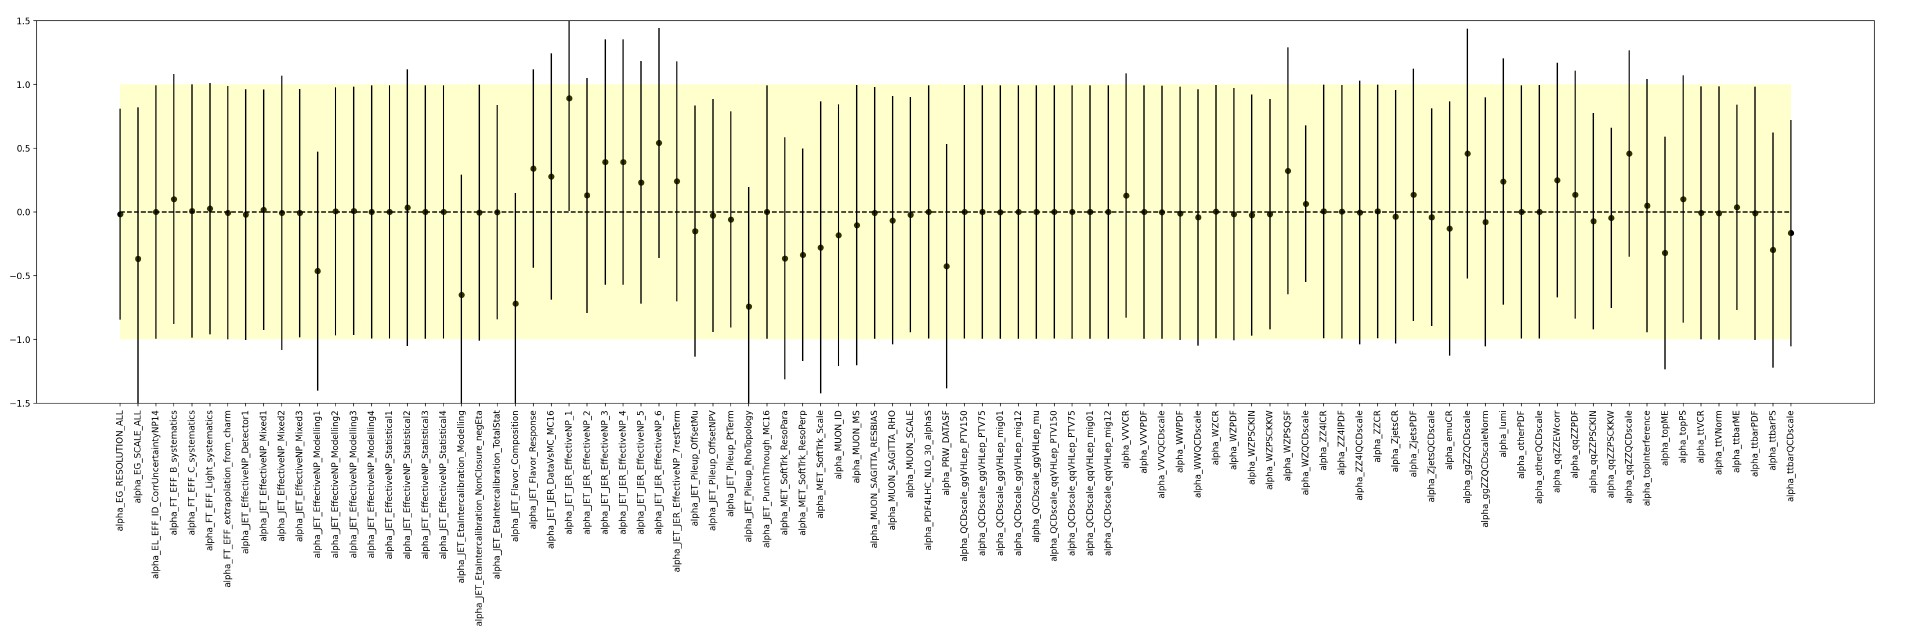
\includegraphics[width=0.98\linewidth]{figures/ch6-DM/ZHinv-fit-pull.jpg}
    \caption{Pulls of the nuisance parameters from the combined fit to data.}
    \label{fig:pull-fit}
\end{figure}

From the fit, the signal strength is determined to be 
$\mu_s = 0.003 \pm 0.090$. 
The normalization factors for the dominant background processes are found to be 
$\mu_{\text{WZ}} = 0.971 \pm 0.060$ and 
$\mu_{e\mu} = 0.921 \pm 0.103$. 

The uncertainties on the best-fit value of 
$\mathcal{B}(\text{H} \to \text{inv.})$ are also evaluated. 
Table~\ref{tab:branching-Hins-syst} summarizes the contributions from both theoretical and experimental uncertainties to 
$\Delta\mathcal{B}(\text{H} \to \text{inv.})$.
\begin{table}[!htbp]
\centering
\begin{tabular}{l r}
\hline\hline
Uncertainty source & $\Delta\mathcal{B}$ [\%] \\
\hline

Statistical uncertainty & 5.1 \\

Systematic uncertainties & 7.4 \\
\quad Theory uncertainties & 4.9 \\
\quad\quad Signal modelling & 0.4 \\
\quad\quad $\text{ZZ}$ modelling & 4.4 \\
\quad\quad Non-$\text{ZZ}$ background modelling & 2.1 \\

\quad Experimental uncertainties (excl. MC stat.) & 4.6 \\
\quad\quad Luminosity, pile-up & 1.5 \\
\quad\quad Jets, $E_{\text{T}}^{\text{miss}}$ & 4.0 \\
\quad\quad Flavour tagging & 0.4 \\
\quad\quad Electrons, muons & 1.2 \\

\quad MC statistical uncertainty & 1.6 \\

\hline
Total uncertainty & 9.0 \\
\hline\hline
 
\end{tabular}
\caption{Summary of the uncertainties $\Delta\mathcal{B}$ on the best-fit $\Delta\mathcal{B} (\text{H} \to \text{inv.})$, obtained by fixing the corresponding nuisance parameters to their best-fit values, and subtracting the square of the resulting uncertainty from the square of the total uncertainty to evaluate $\Delta\mathcal{B}^2$. The statistical uncertainty component is obtained by fixing all nuisance parameters to their best-fit values. 
%Note that the total uncertainty does not equal the sum of the individual contributions added in quadrature due to correlations between the systematic uncertainties.
}
\label{tab:branching-Hins-syst}
\end{table}

Based on the fit results, the observed upper limit on the Higgs boson branching fraction to invisible particles, obtained using all control regions, is 
$\mathcal{B}(\text{H} \to \text{inv.}) = 18.7\%$ at 95\% confidence level (CL). The predicted limit on $\mathcal{B}(\text{H} \to \text{inv.})$ is 19.0\%.
This corresponds to an improvement of more than 50\% in sensitivity compared to the result obtained using partial Run~2 data.

\subsection{Limits from Simplified DM Models in the Mono-$\text{Z}$ Channel}
\label{sec:Mono-Z-search}

The Mono-$\text{Z}$ limits are derived using a simultaneous fit to the $3\ell$, $4\ell$, and $e\mu$ control regions, with floating normalization factors applied to the $\text{WZ}$ and non-resonant backgrounds. The $\text{Z}$+jets, $t\bar{t}\text{V}$, and $\text{VVV}$ backgrounds are estimated entirely from MC simulations. 

The primary fitting discriminant is the $m_{\text{T}}^{\text{ZZ}}$ variable. 
This observable is also used in the non-resonant CR, while the 
$E_{\text{T}}^{\text{miss}}$ distribution is employed in the $3\ell$ ($\text{WZ}$) 
and $4\ell$ ($\text{ZZ}$) CRs. 

Figure~\ref{fig:mon-z-mT} shows the pre-fit and post-fit 
$m_{\text{T}}^{\text{ZZ}}$ distributions for data and MC predictions 
of the DM signal hypothesis (with $m_\chi = 150~\text{GeV}$ and 
$m_{\text{med}} = 900~\text{GeV}$) and the background processes in the SR. 
No significant excess of data over the predicted background is observed.

Only events with $m_{\text{T}}^{\text{ZZ}} > 200~\text{GeV}$ are included in the fit to further suppress SM background contributions from regions not relevant to the targeted signals. 
Systematic uncertainties are evaluated for both signal and background processes; however, those with an impact of 1\% or less are excluded from the fit. 
Validation studies show that this choice results in a negligible change in the derived limits while significantly improving computational efficiency.

\begin{figure}[!htbp]
    \centering
    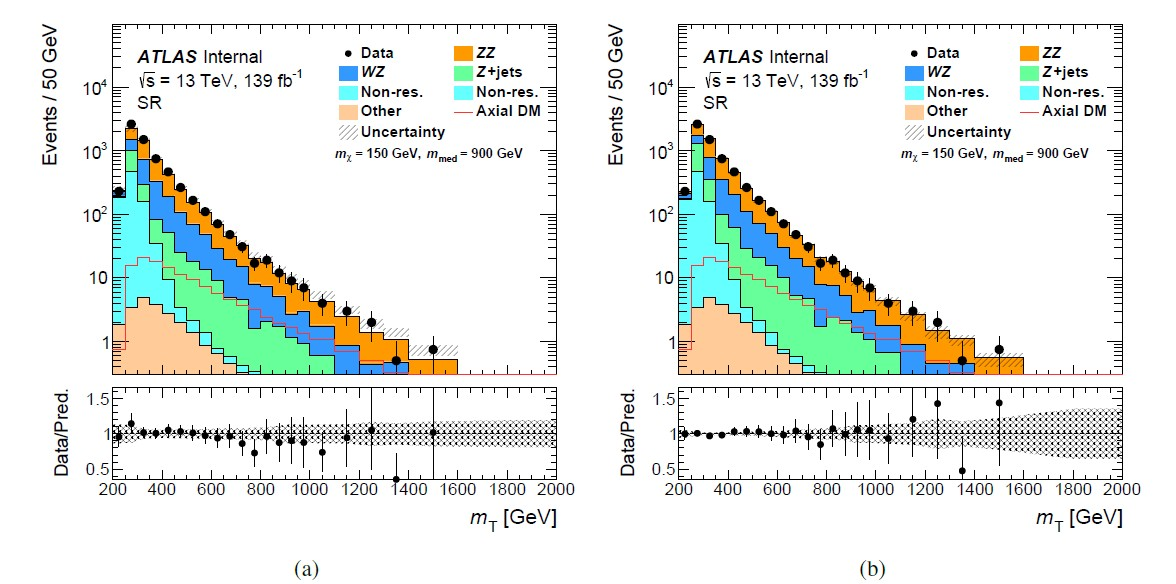
\includegraphics[width=0.98\linewidth]{figures/ch6-DM/Mono-Z-mT.jpg}
    \caption{The $m_{\text{T}}^{\text{ZZ}}$ distribution in the SR: (a) pre-fit and (b) post-fit.}
    \label{fig:mon-z-mT}
\end{figure}

The exclusion limits in the $(m_\chi, m_{\text{med}})$ parameter space are shown in Figure~\ref{fig:mono-Z-limit} for an axial-vector mediator (panel~a) and a vector mediator (panel~b). 
Previous ATLAS results based on $36.1~\text{fb}^{-1}$ of Run~2 data are also indicated for comparison. 
The current analysis significantly enlarges the excluded region relative to these earlier results.

\begin{figure}[!htbp]
    \centering
    \subfloat[]{
    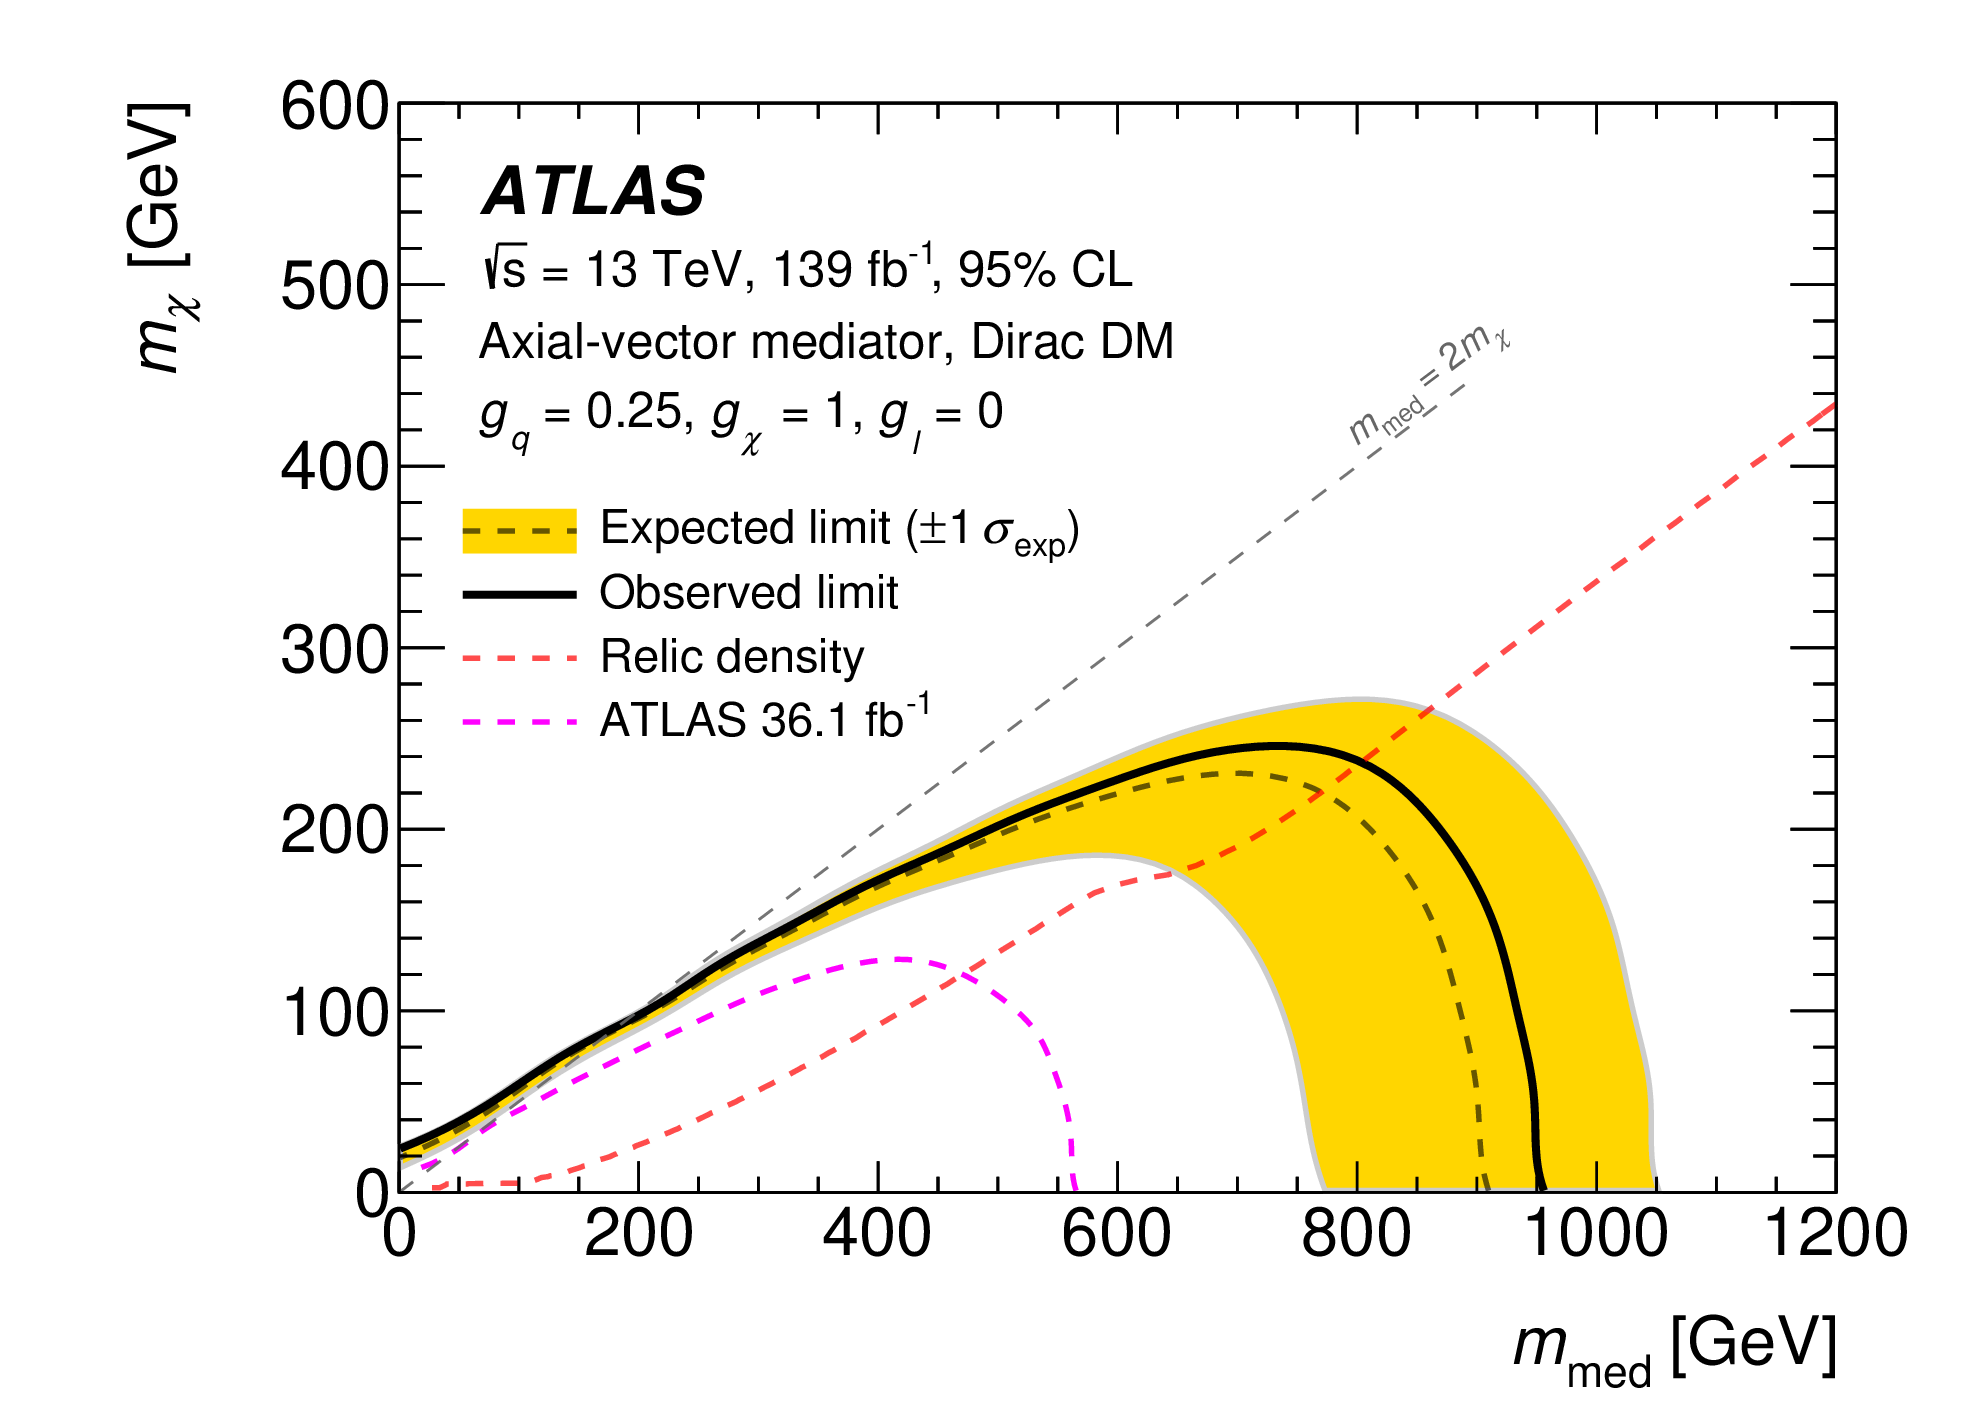
\includegraphics[width=0.49\linewidth]{figures/ch6-DM/fig_04a.png}}
    \subfloat[]{
    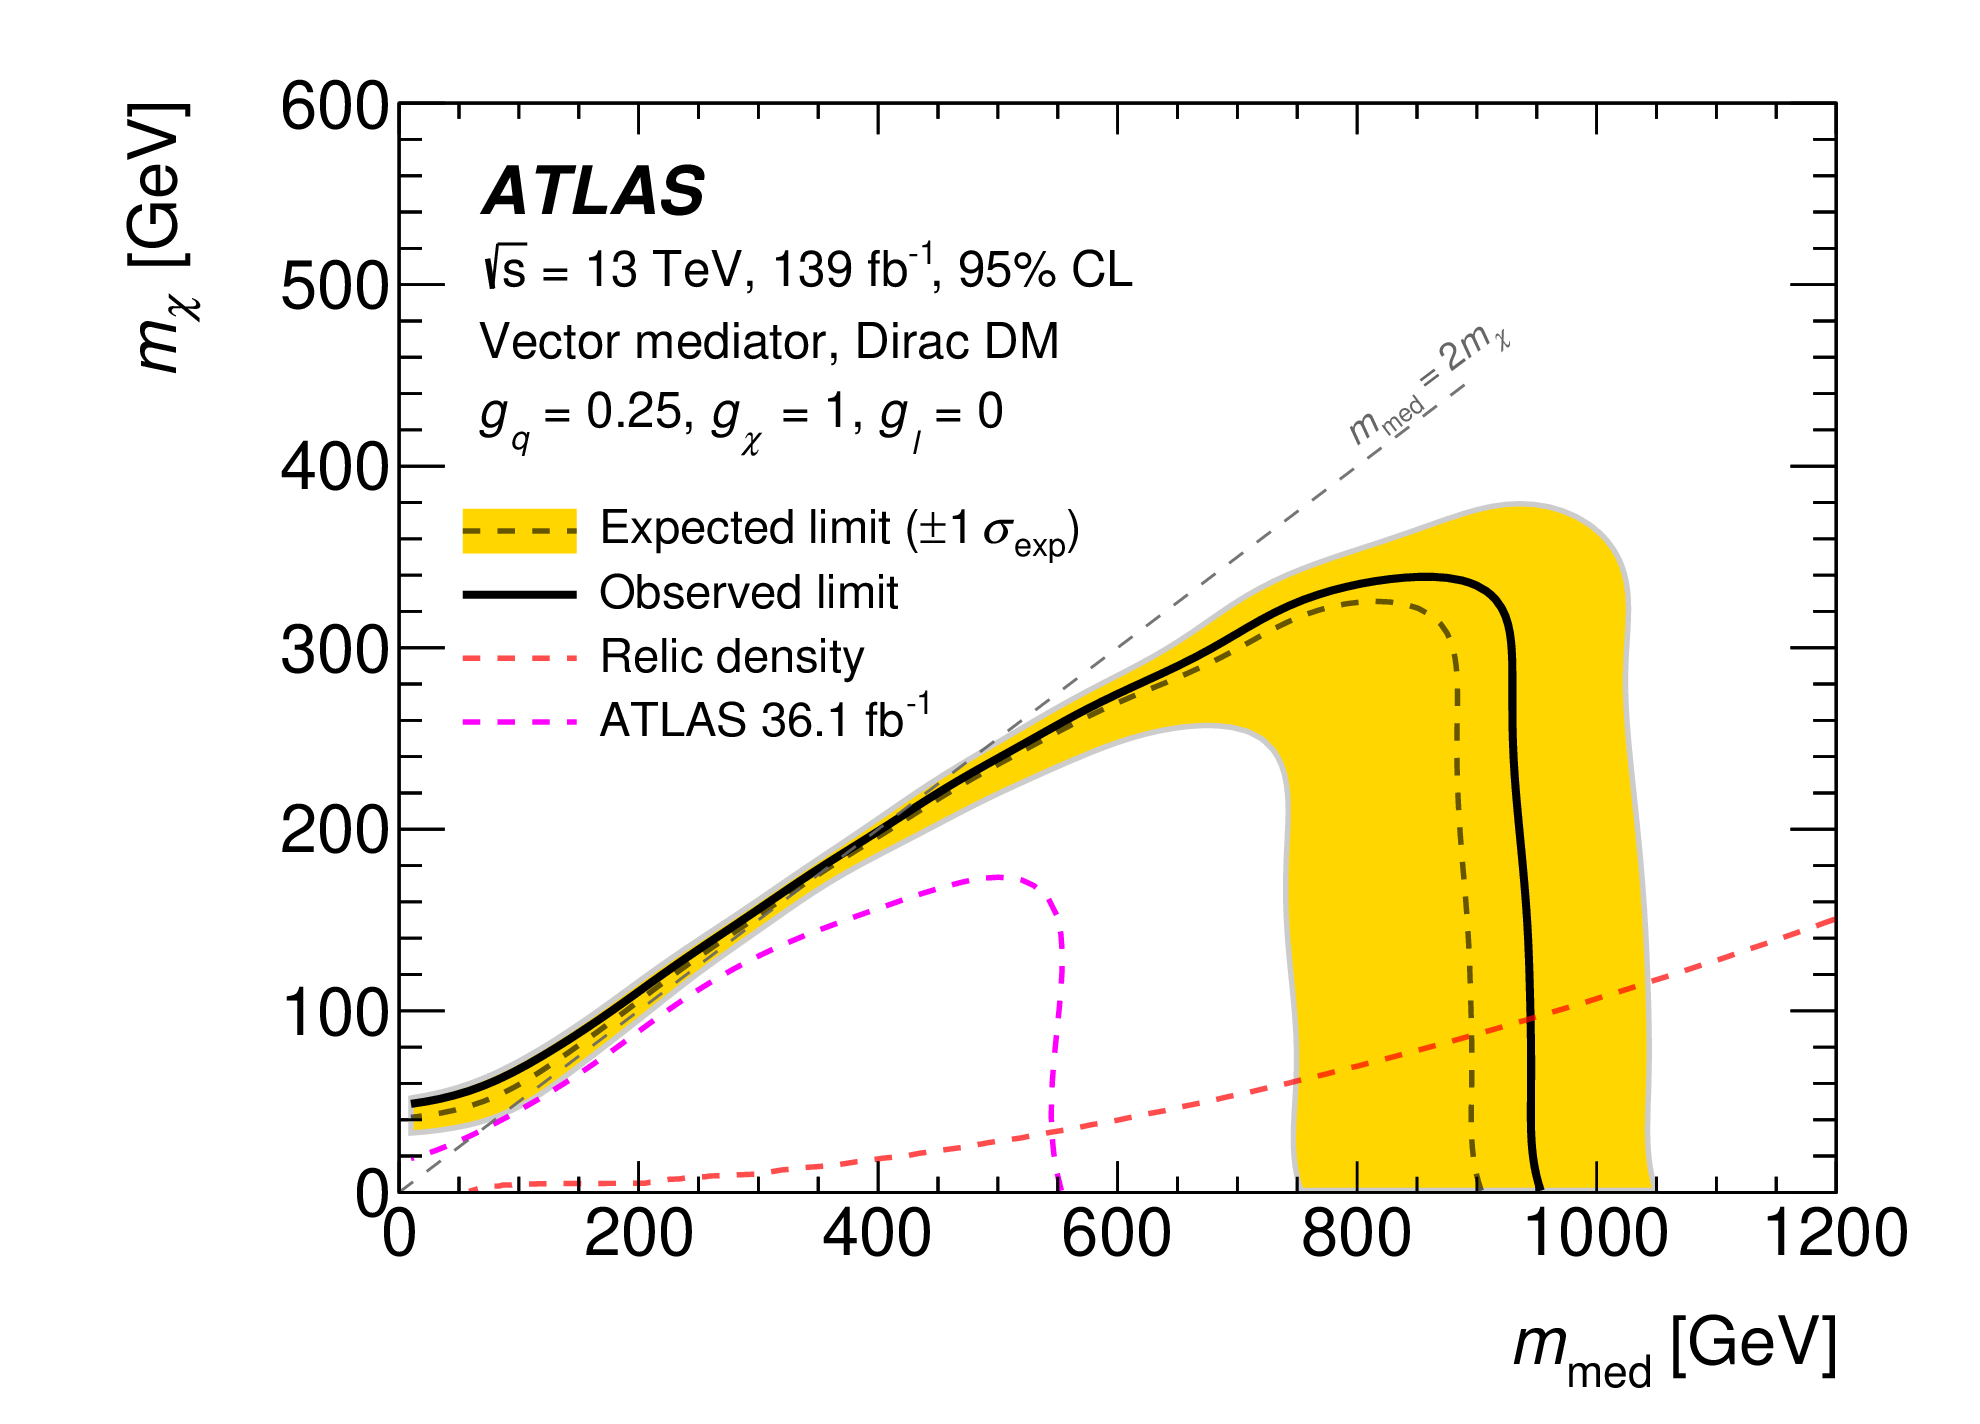
\includegraphics[width=0.49\linewidth]{figures/ch6-DM/fig_04b.png}}      
    \caption{Exclusion limits for simplified DM models with $g_\chi = 1.0$, $g_q = 0.25$, and $g_\ell = 0$, when assuming 
    (a) an axial-vector mediator or (b) a vector mediator. 
    The region below the solid black line is excluded at the 95\% CL. The dashed black line indicates the expected limit in the absence of signal, and the yellow band the corresponding $\pm 1\sigma$ uncertainty band. The dashed red line labelled `Relic density' corresponds to combinations of DM and mediator mass values that are consistent with a DM density of $\Omega h^2 = 0.118$ and a standard thermal history, as computed in Ref.~\cite{Albert:2017onk}. Below the line, annihilation processes described by the simplified model mostly predict too high a relic density, while regions with too low a relic density are mostly found for $m_{\text{med}}$ closer to the DM mass. The dashed
    magenta line indicates the previous ATLAS result from the $36.1~\text{fb}^{-1}$ Run 2 data.}
    \label{fig:mono-Z-limit}
\end{figure}

\subsection{Exclusion Limits for the 2HDM+$a$ Model}
\label{sec:2HDMa-search}

The $\text{Z} + E_{\text{T}}^{\text{miss}}$ channel provides the highest sensitivity over a large fraction of the parameter space for 2HDM+$a$ searches.
The observed $m_{\text{T}}^{\text{ZZ}}$ spectrum in data is fitted to the 2HDM+$a$ signal hypothesis together with the SM background predictions to set exclusion limits in the model parameter space. 
In this model, the two Higgs doublets are CP-conserving and of Type-II, with the lighter scalar identified as the observed 125~GeV Higgs boson. 

Four benchmark scenarios are probed in various parameter planes as functions of the mass of the pseudoscalar Higgs boson, $m_A$, the mass of the additional pseudoscalar, $m_a$, the ratio of the vacuum expectation values of the two Higgs doublets, $\tan\beta$, and $\sin\theta$, where $\theta$ is the mixing angle between the two CP-odd weak spin-0 eigenstates. 

Following the recommendations in Ref.~\cite{Abe:2018emu}, eight scans of the parameter space are performed for the 2HDM+$a$ model, imposing the requirement $m_A = m_{\text{H}} = m_{H^\pm}$. 
The four primary free parameters investigated in this search are $m_a$, $m_A$, $\tan\beta$, and $\sin\theta$.

Exclusion limits are derived within the context of the 2HDM+$a$ model for different parameter choices and in several parameter planes. 
Figure~\ref{fig:2HDMa-limit} shows the two-dimensional exclusion contours for $\sin\theta = 0.35$ and 0.7: 
(a) and (b) in the $(m_a, m_A)$ plane for $\tan\beta = 1.0$, 
(c) and (d) in the $(m_a, \tan\beta)$ plane, and 
(e) and (f) in the $(m_A, \tan\beta)$ plane. 
The remaining model parameters used in each scan are indicated in the corresponding plots. 

Figure~\ref{fig:2HDMa-sintheta-limit} presents the exclusion limits on $\sin\theta$ for 2HDM+$a$ signals with $\tan\beta = 1.0$ and $m_\chi = 10~\text{GeV}$. 
Panel (a) shows the limit for $m_a = 200~\text{GeV}$ and $m_A = 600~\text{GeV}$, while panel (b) corresponds to $m_a = 350~\text{GeV}$ and $m_A = 1000~\text{GeV}$.

The region enclosed by the solid black line and hashed black contour is excluded at 95\% confidence level (CL). 
The solid blue line indicates the expected limit in the absence of signal, while the dashed blue lines represent the corresponding $\pm1\sigma$ uncertainty band. 
The dashed magenta lines show the limits obtained using $36.1~\text{fb}^{-1}$ of data. 
The hashed red area denotes regions where the width of one of the Higgs bosons exceeds 20\% of its mass.

This analysis significantly improves the search sensitivity compared to previous results based on partial Run~2 datasets corresponding to an integrated luminosity of $36.1~\text{fb}^{-1}$.

\begin{figure}[htbp]
    \centering
    \subfloat[]{
    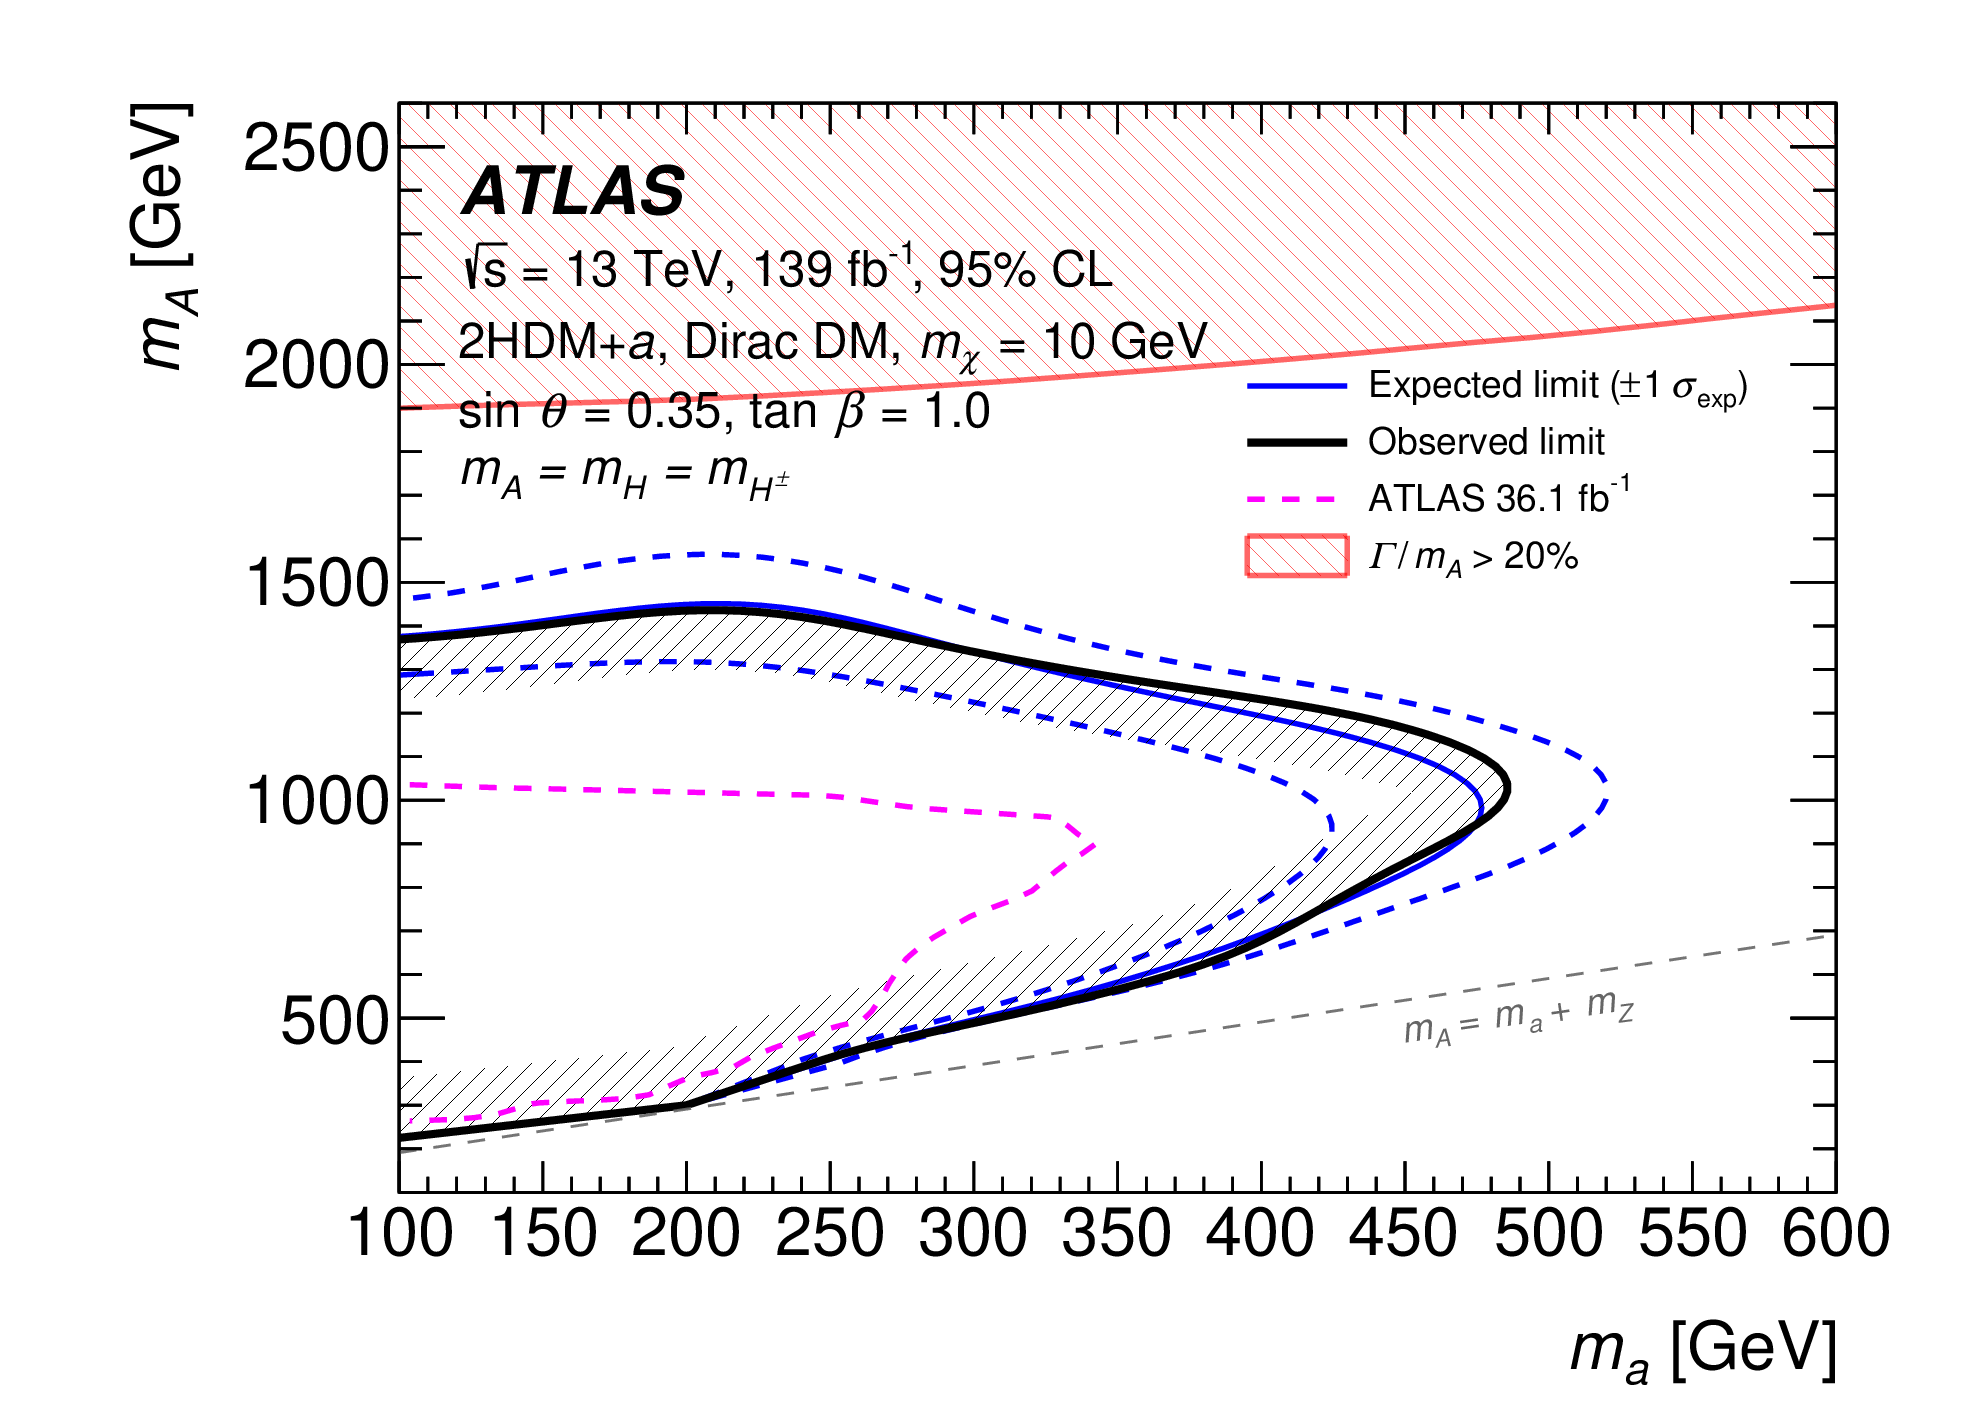
\includegraphics[width=0.49\linewidth]{figures/ch6-DM/fig_05e.png}}
    \subfloat[]{
    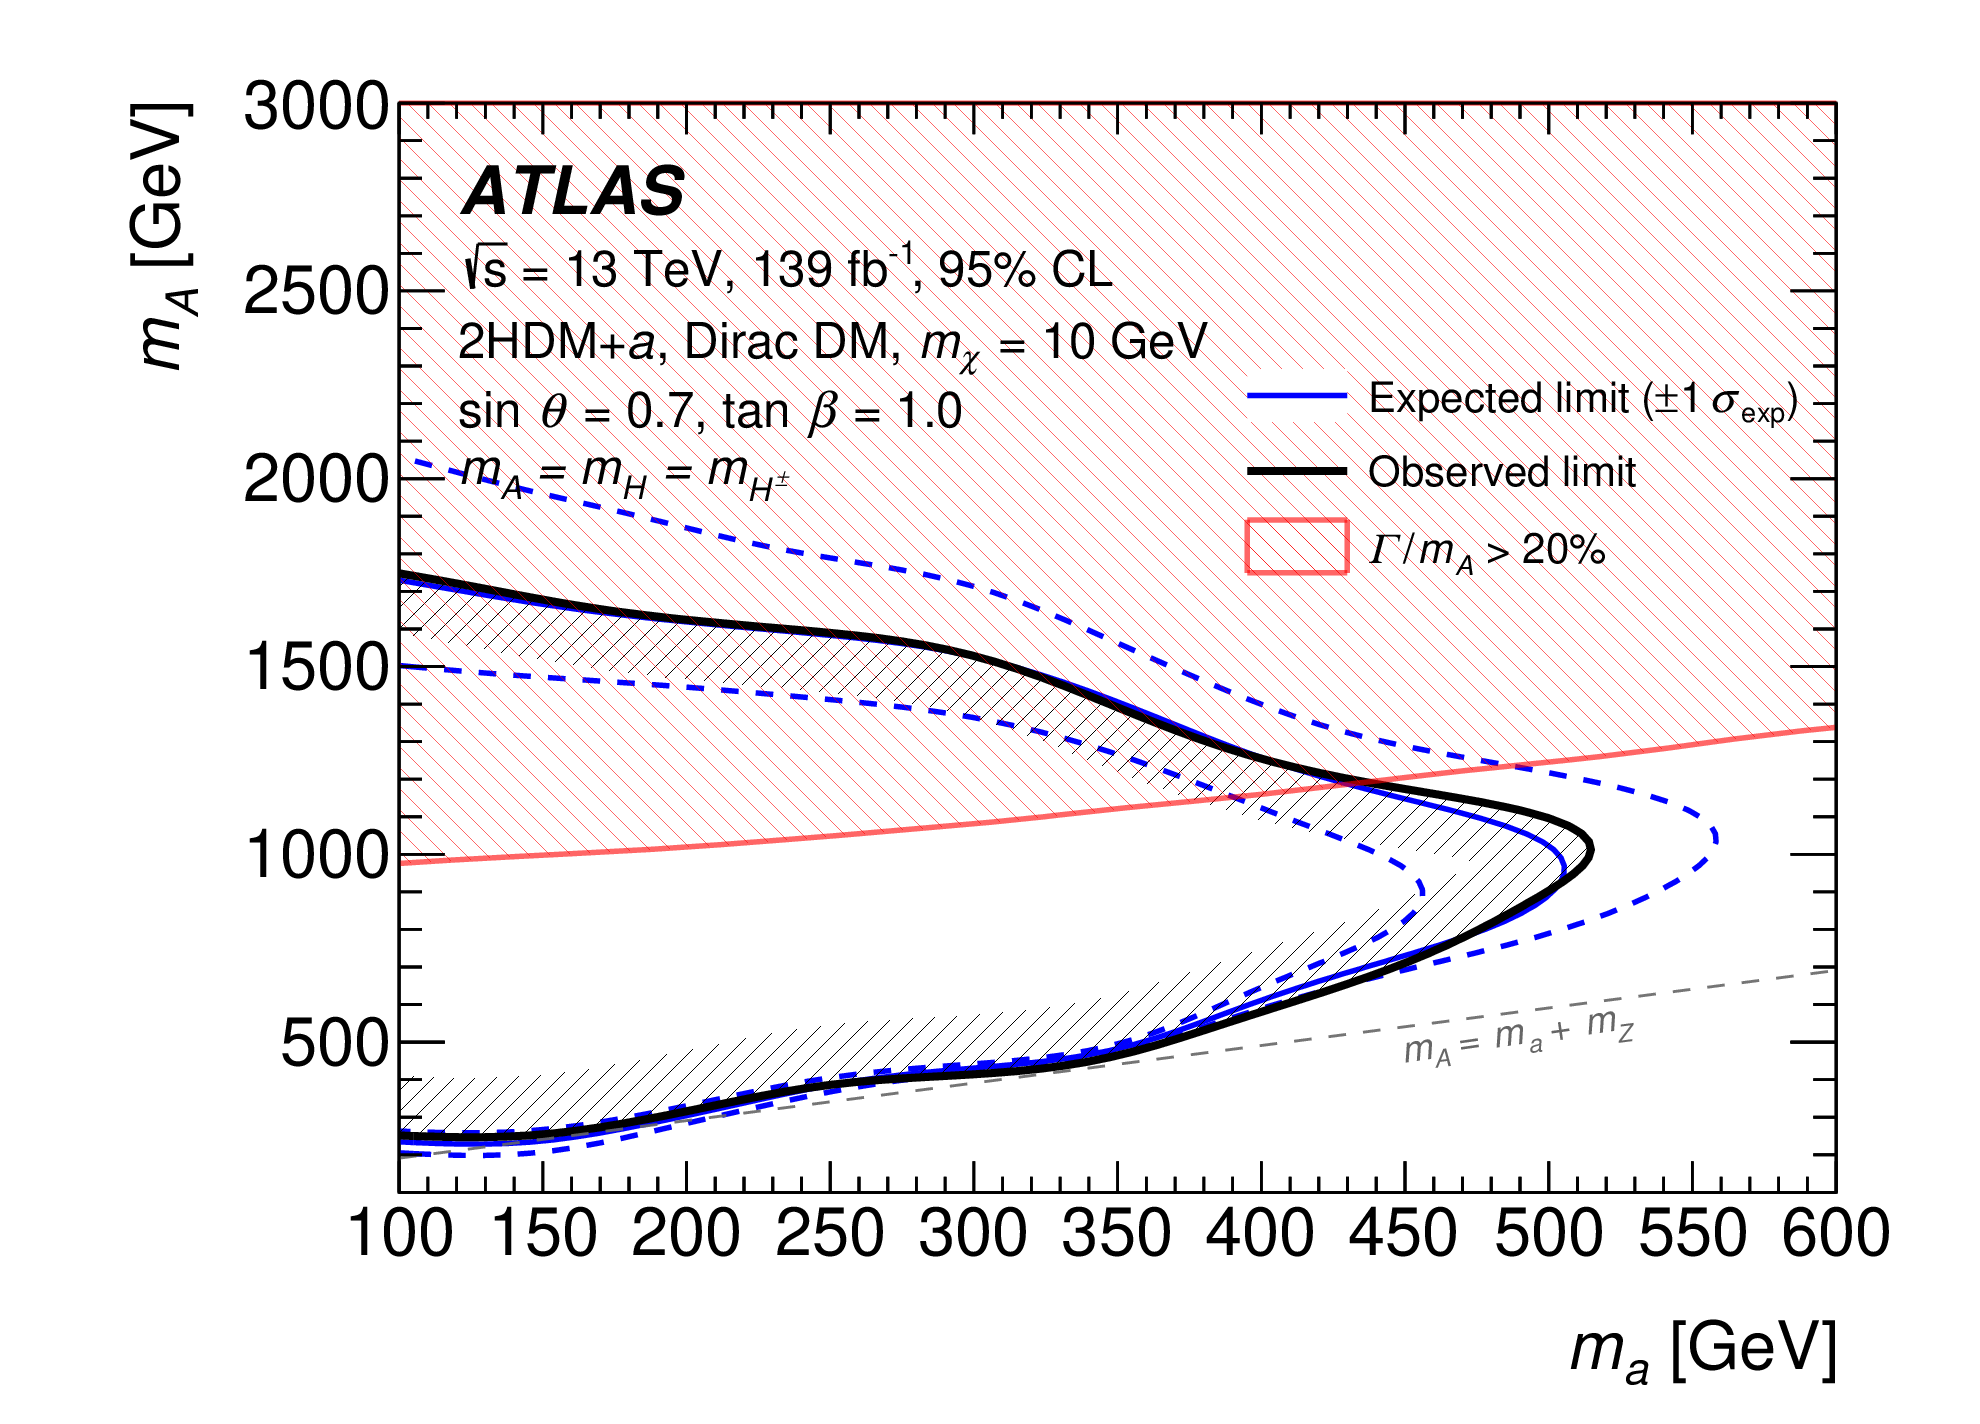
\includegraphics[width=0.49\linewidth]{figures/ch6-DM/fig_05f.png}}  \\    
    \subfloat[]{
    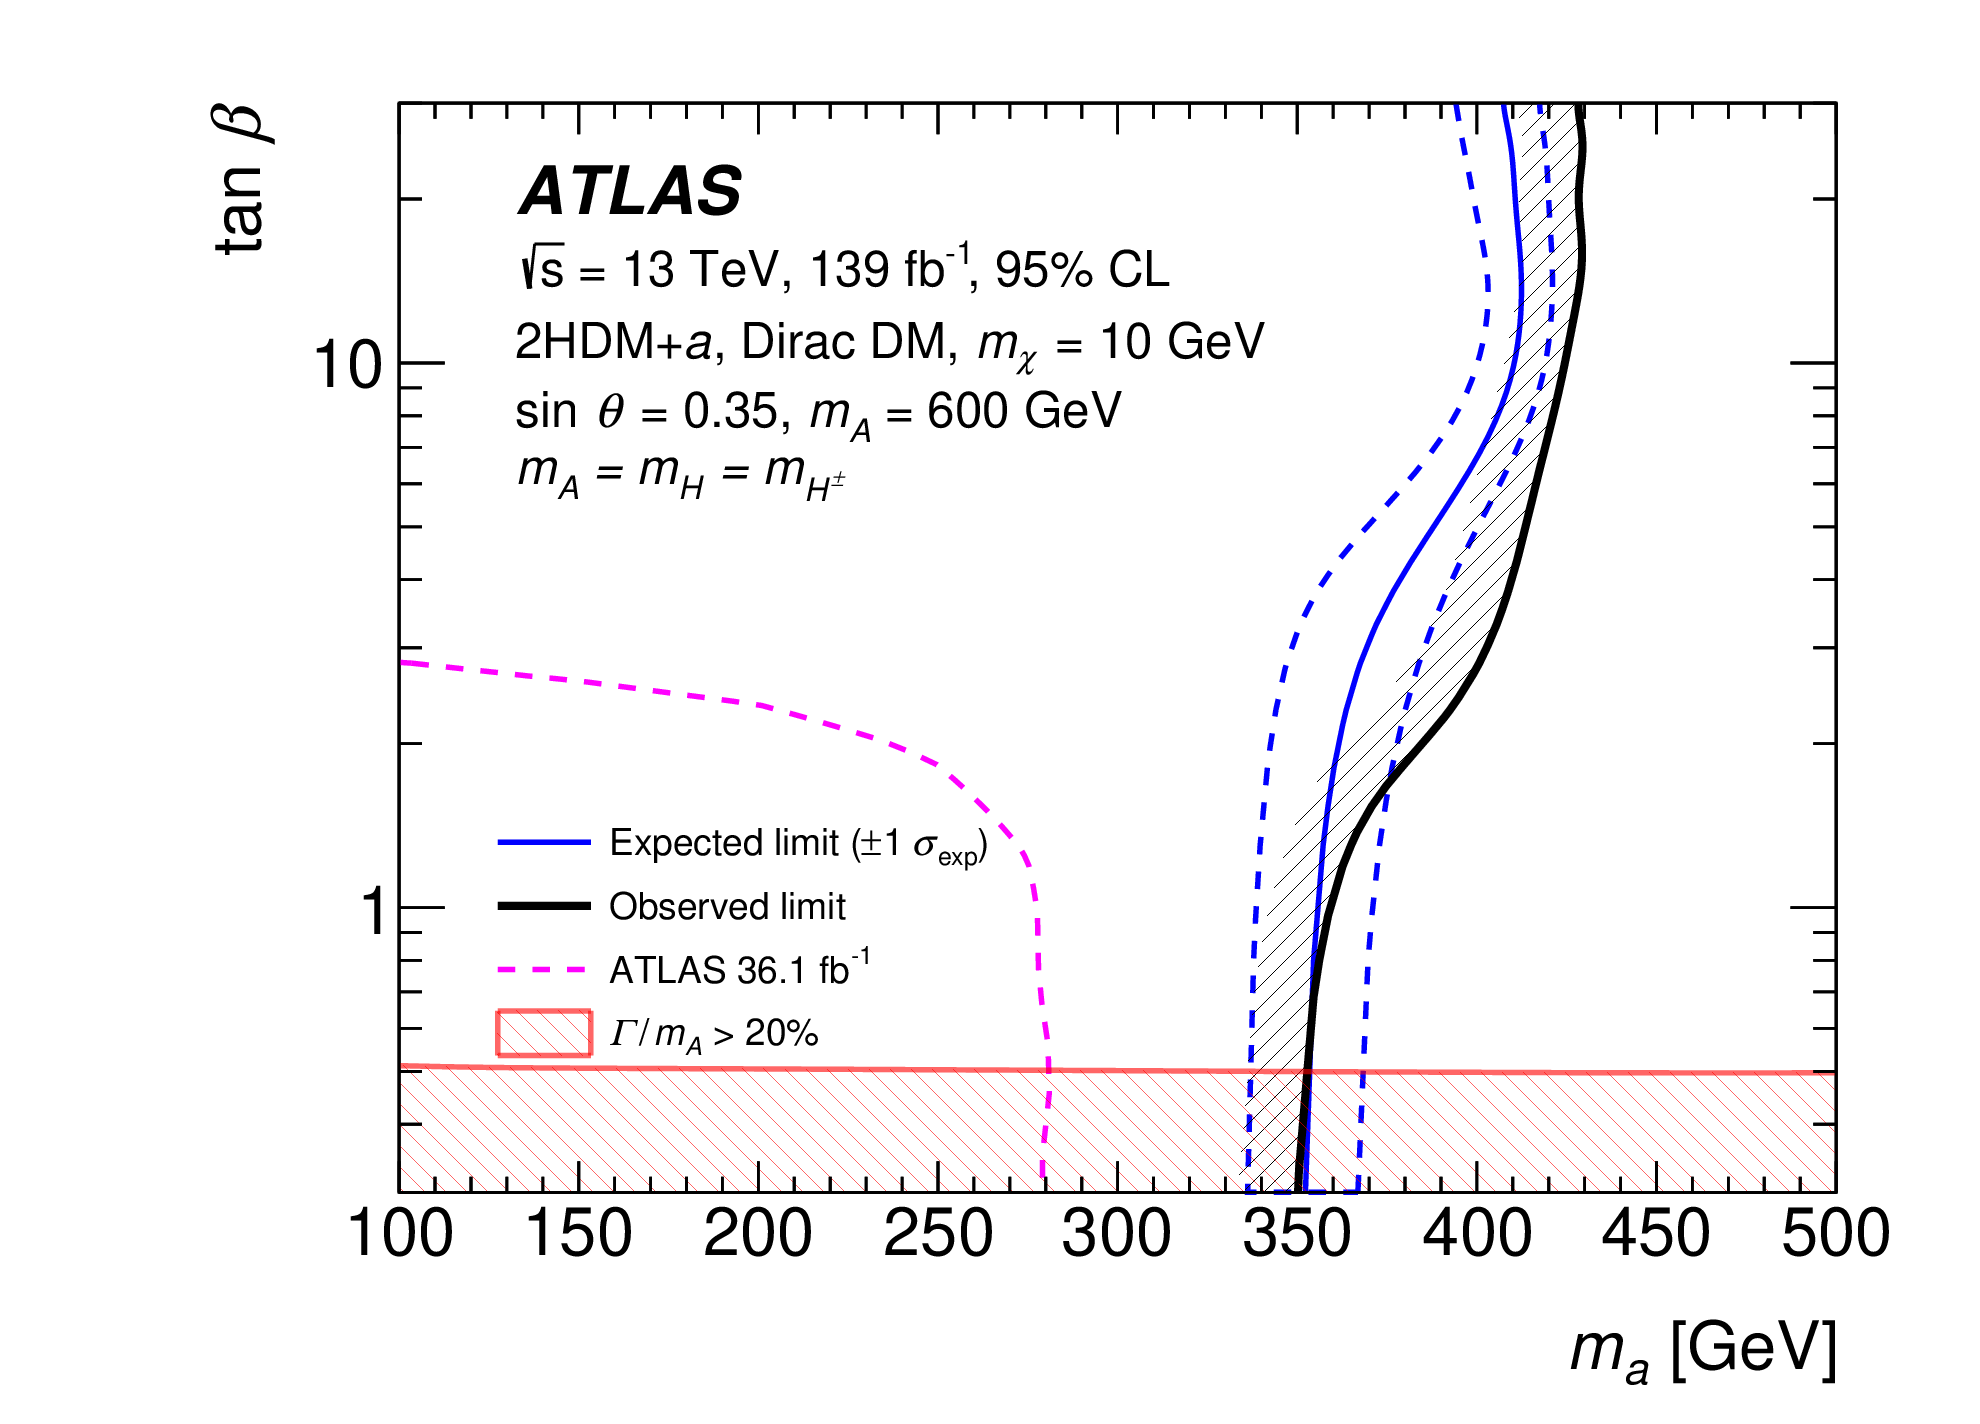
\includegraphics[width=0.49\linewidth]{figures/ch6-DM/fig_05a.png}}
    \subfloat[]{
    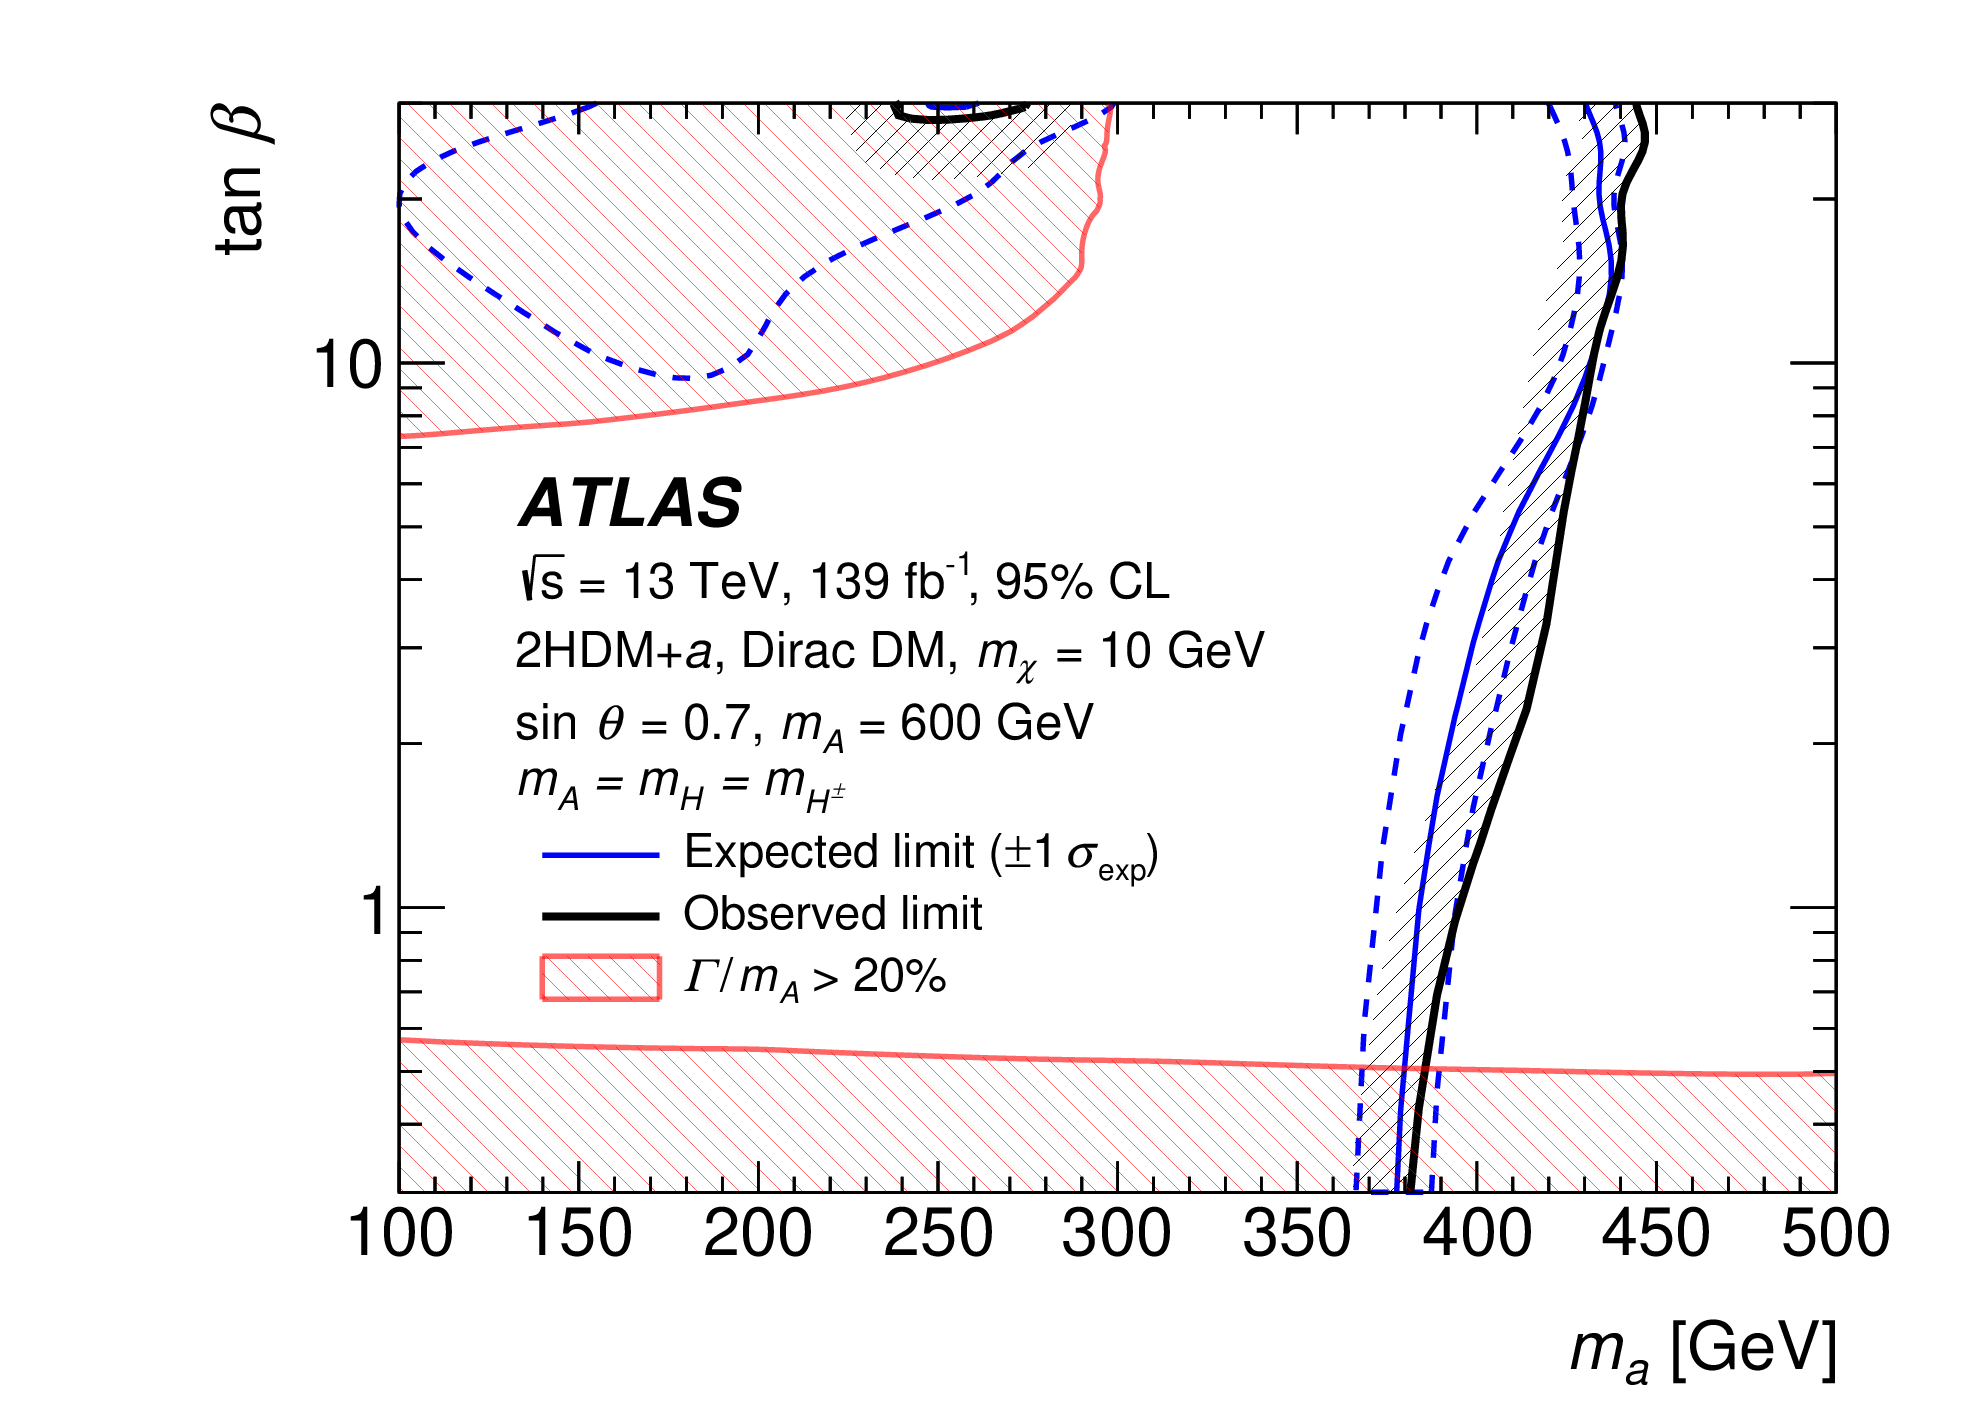
\includegraphics[width=0.49\linewidth]{figures/ch6-DM/fig_05b.png}}  \\
    \subfloat[]{
    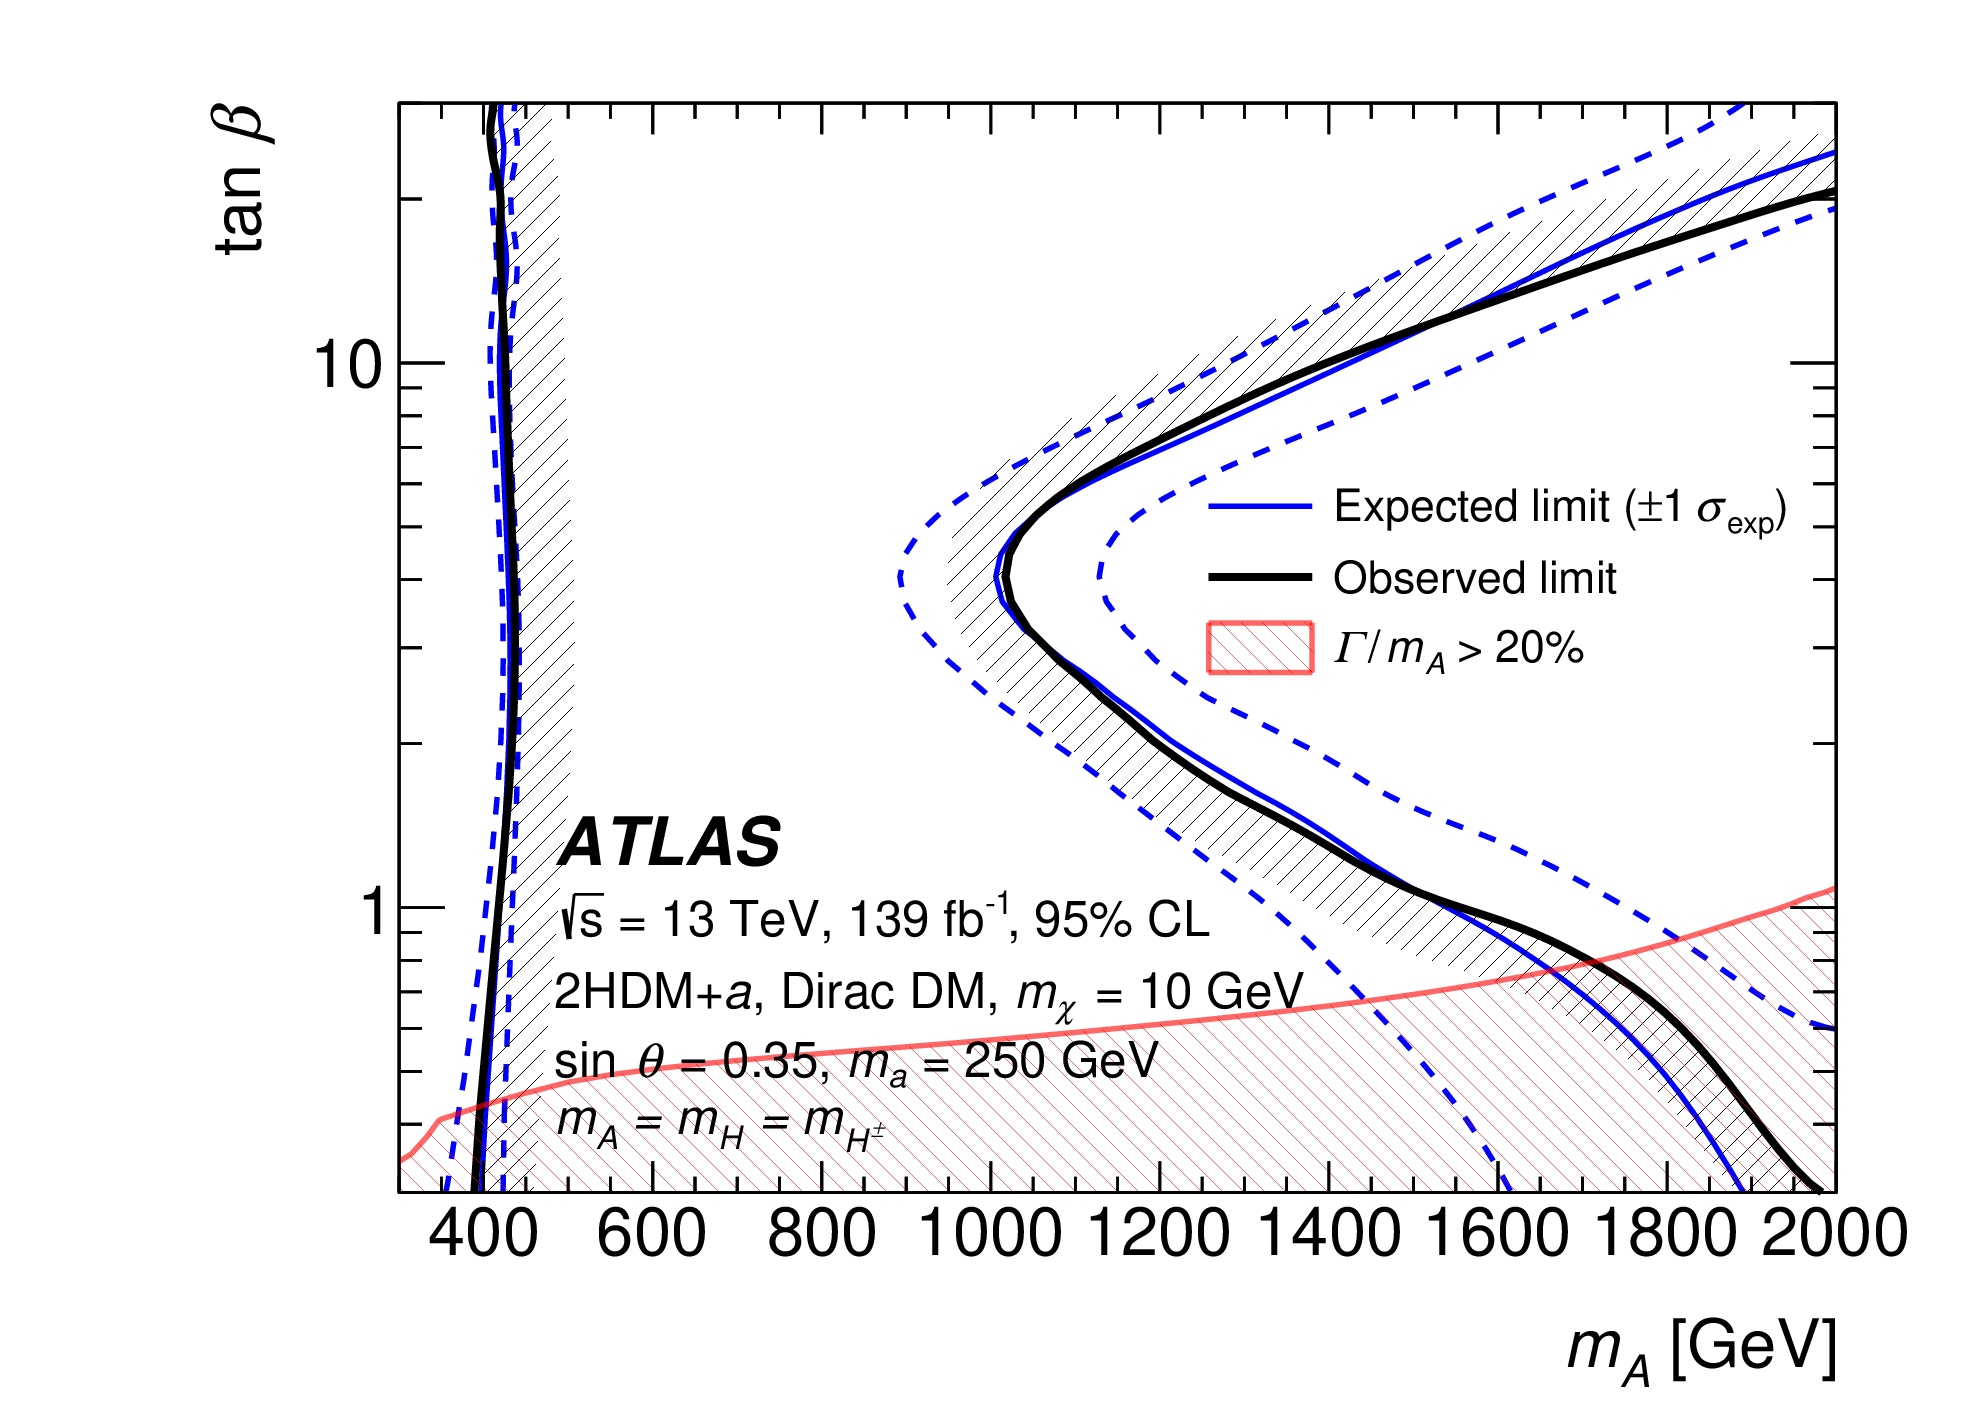
\includegraphics[width=0.49\linewidth]{figures/ch6-DM/fig_05c.png}}
    \subfloat[]{
    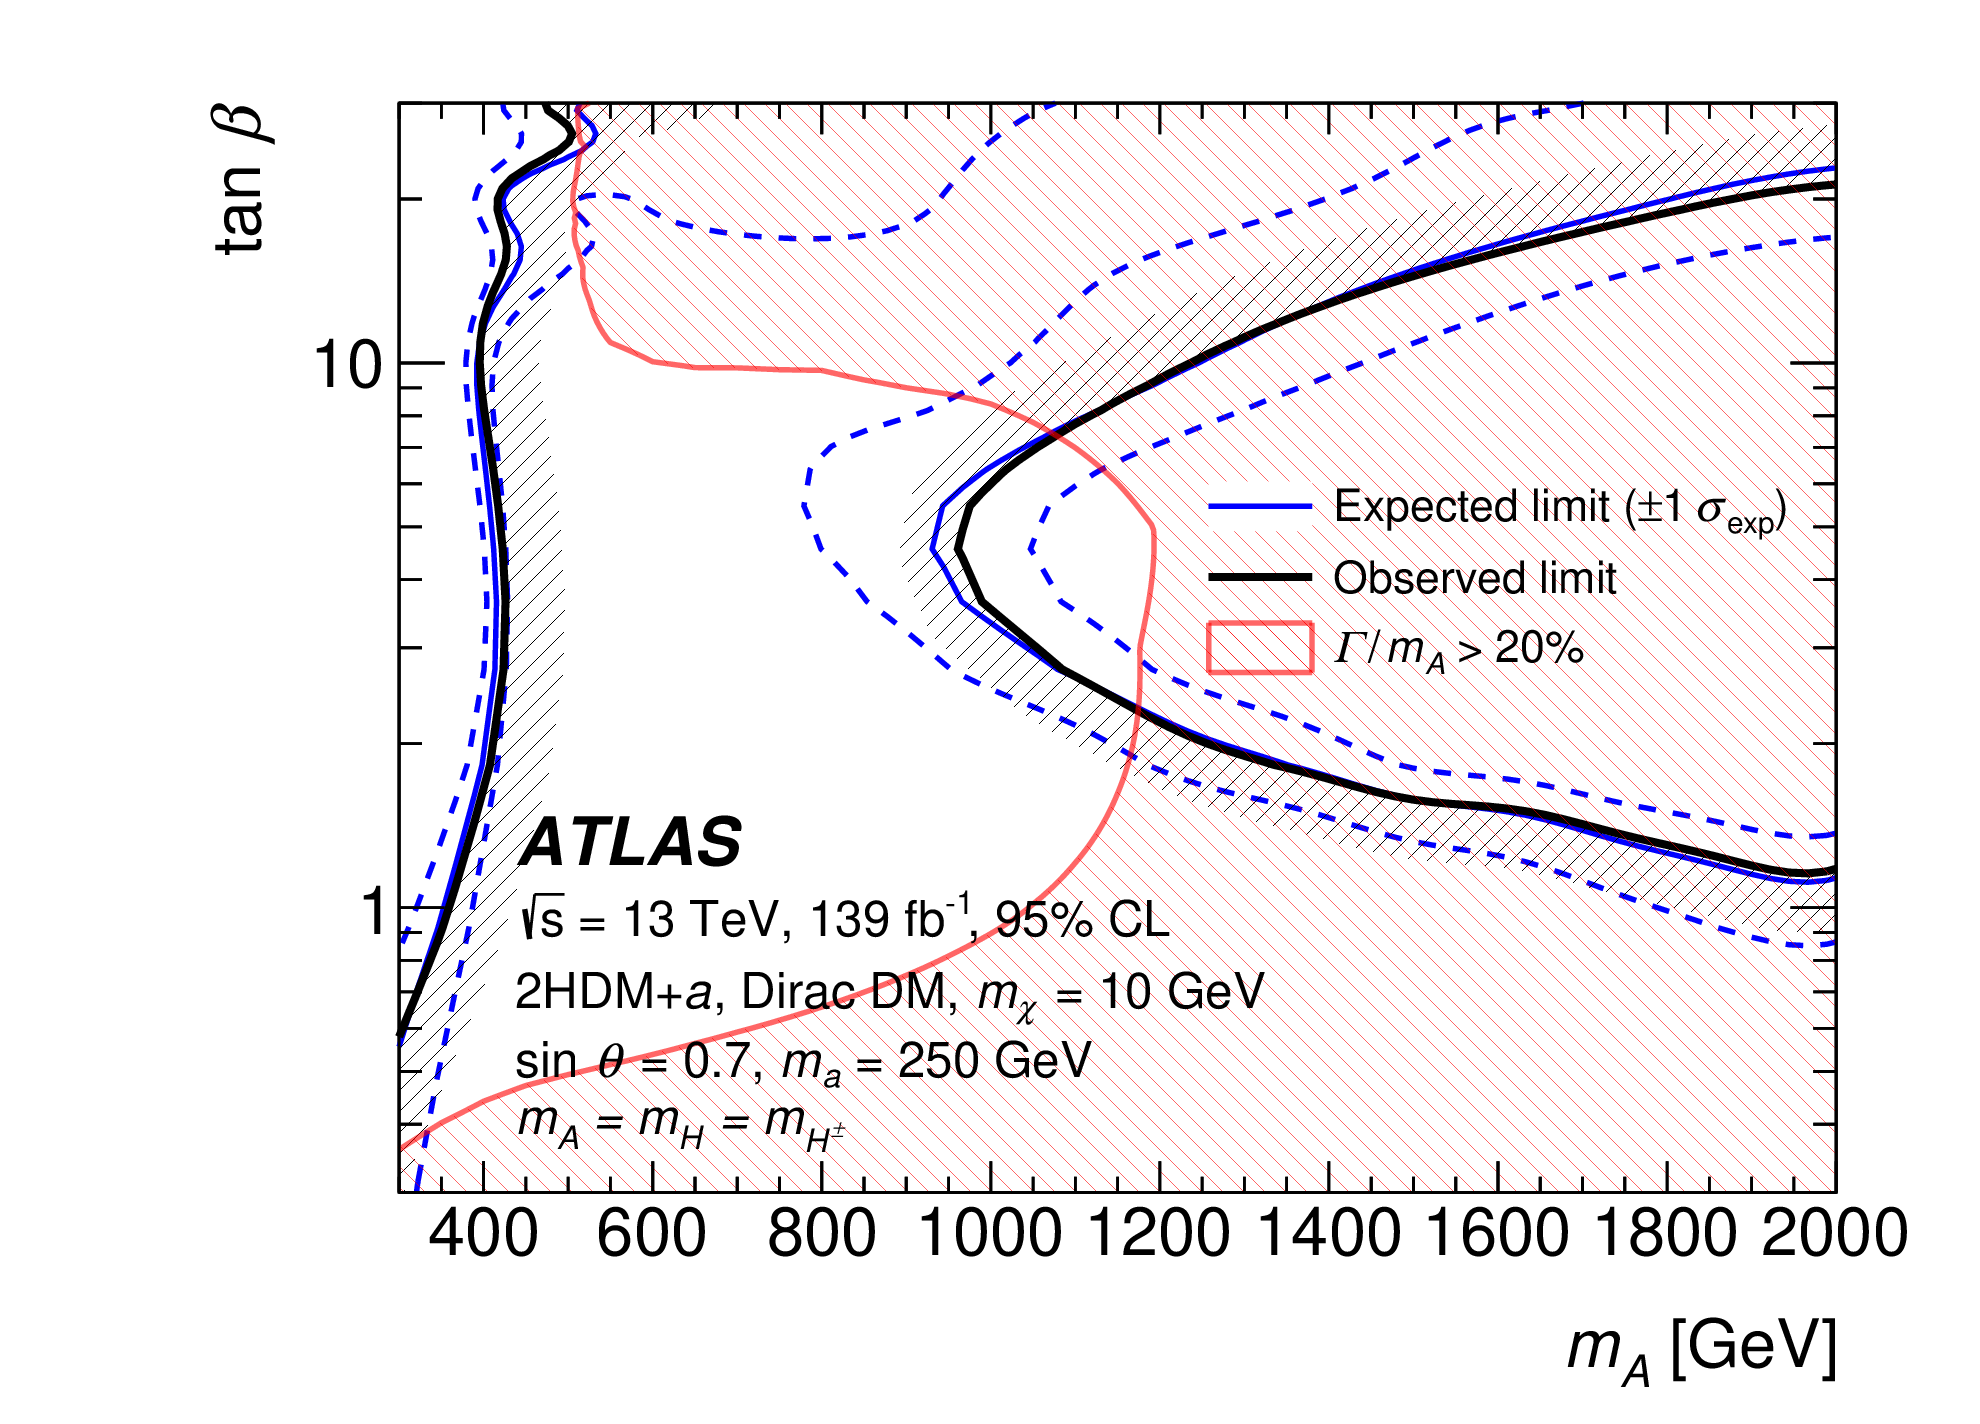
\includegraphics[width=0.49\linewidth]{figures/ch6-DM/fig_05d.png}}  \\        
    \caption{Exclusion limits of the 2HDM+$a$ model with different parameter choices (shown in the plots) and in various planes.
    (a) and (b) show the limits in the ($m_a, m_A$) plane,
    (c) and (d) show the limits in the ($m_a, \tan\beta$) plane, 
    (e) and (f) show the limits in the ($m_A, \tan\beta$) plane, 
    for $\sin\theta = 0.35$ and $0.7$, and other model parameters are indicated in the plots.    
    }
    \label{fig:2HDMa-limit}
\end{figure}

\begin{figure}[!htbp]
    \centering
    \subfloat[]{
    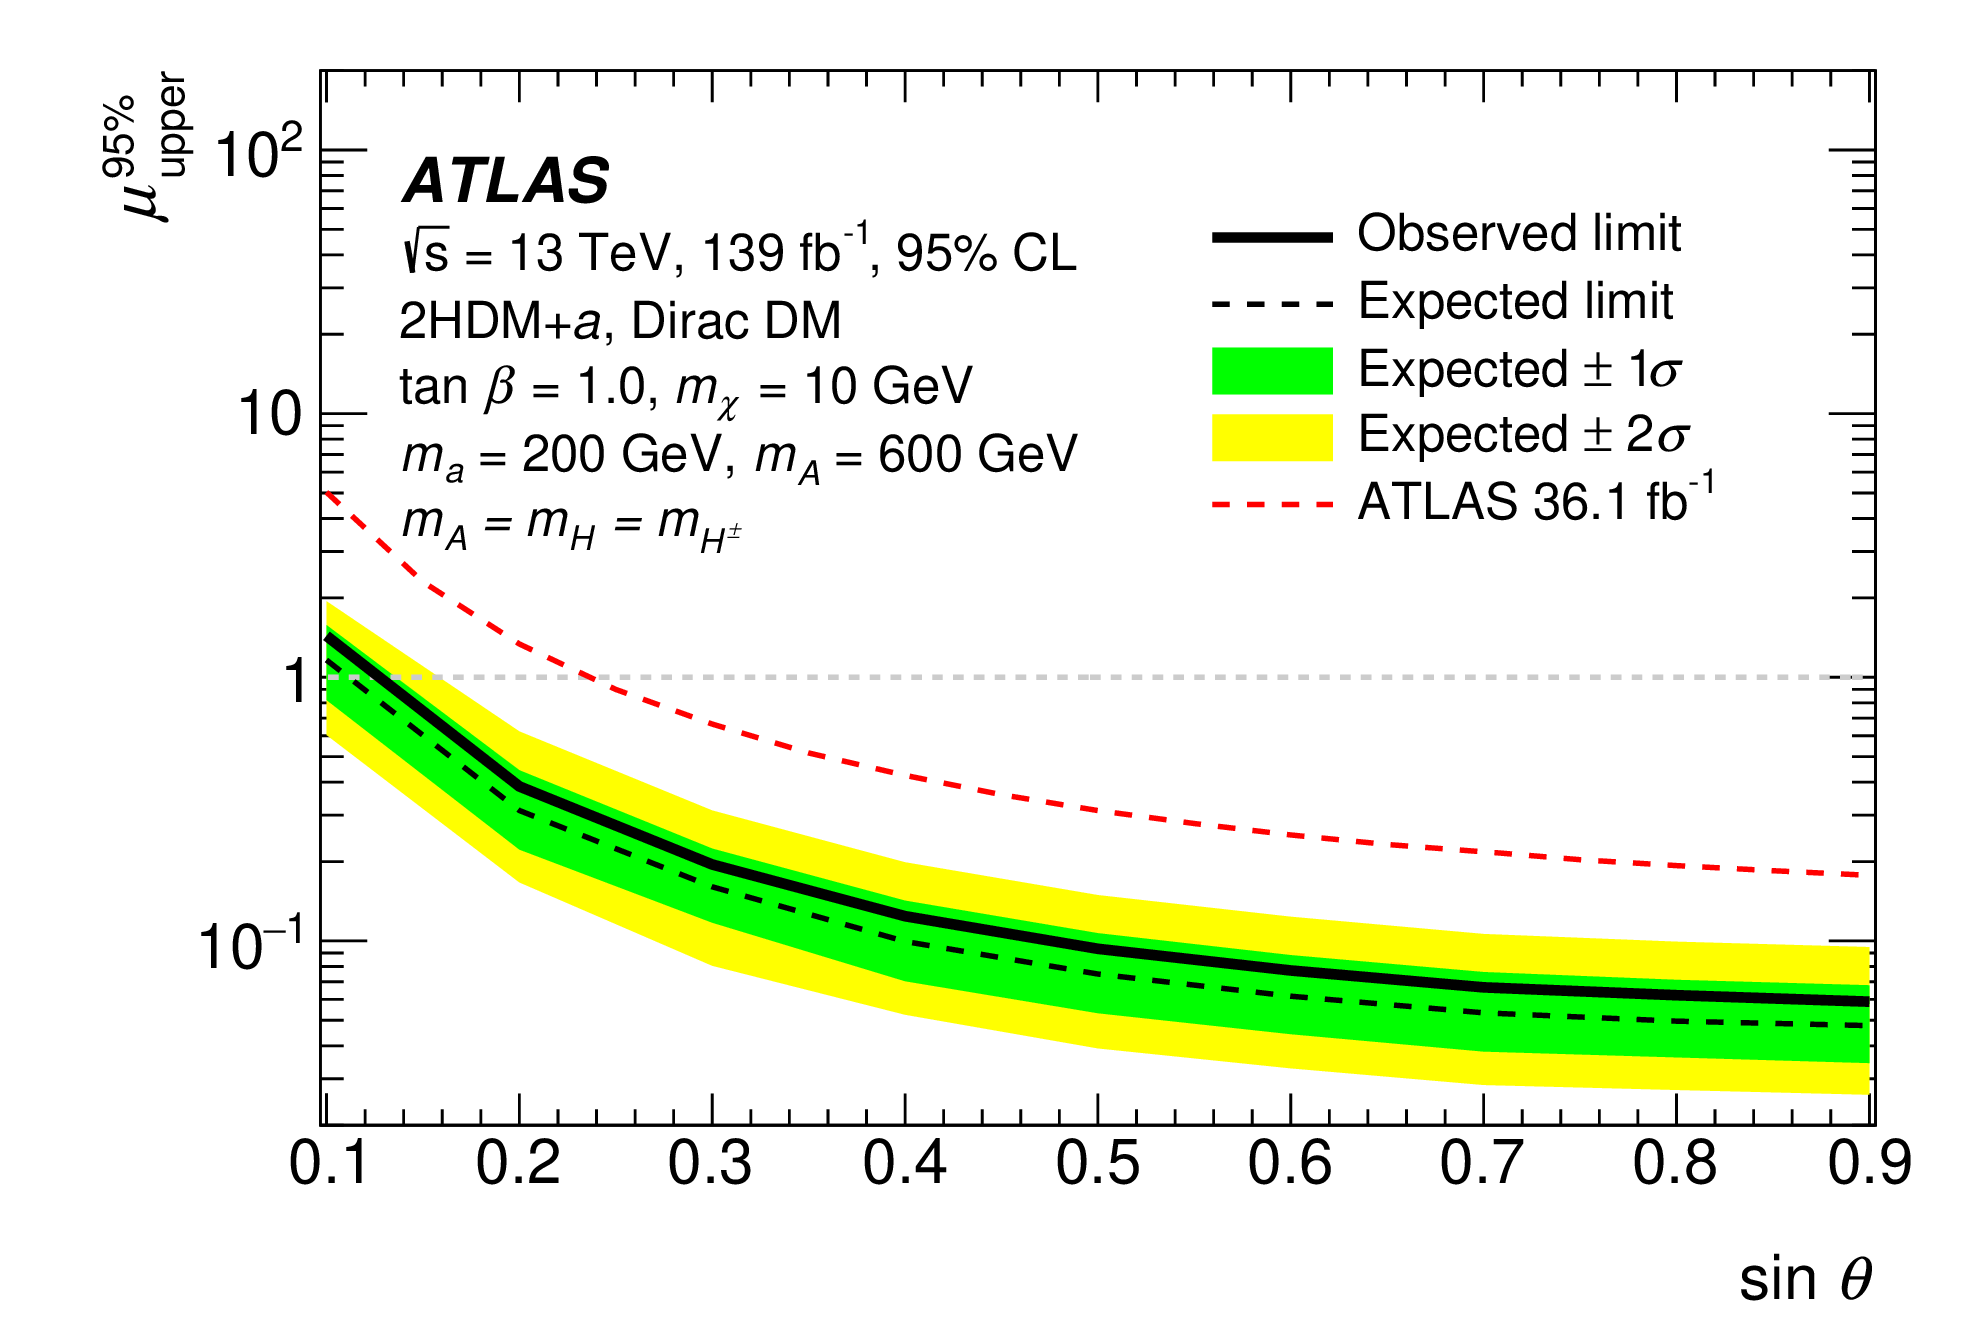
\includegraphics[width=0.49\linewidth]{figures/ch6-DM/fig_06a.png}}
    \subfloat[]{
    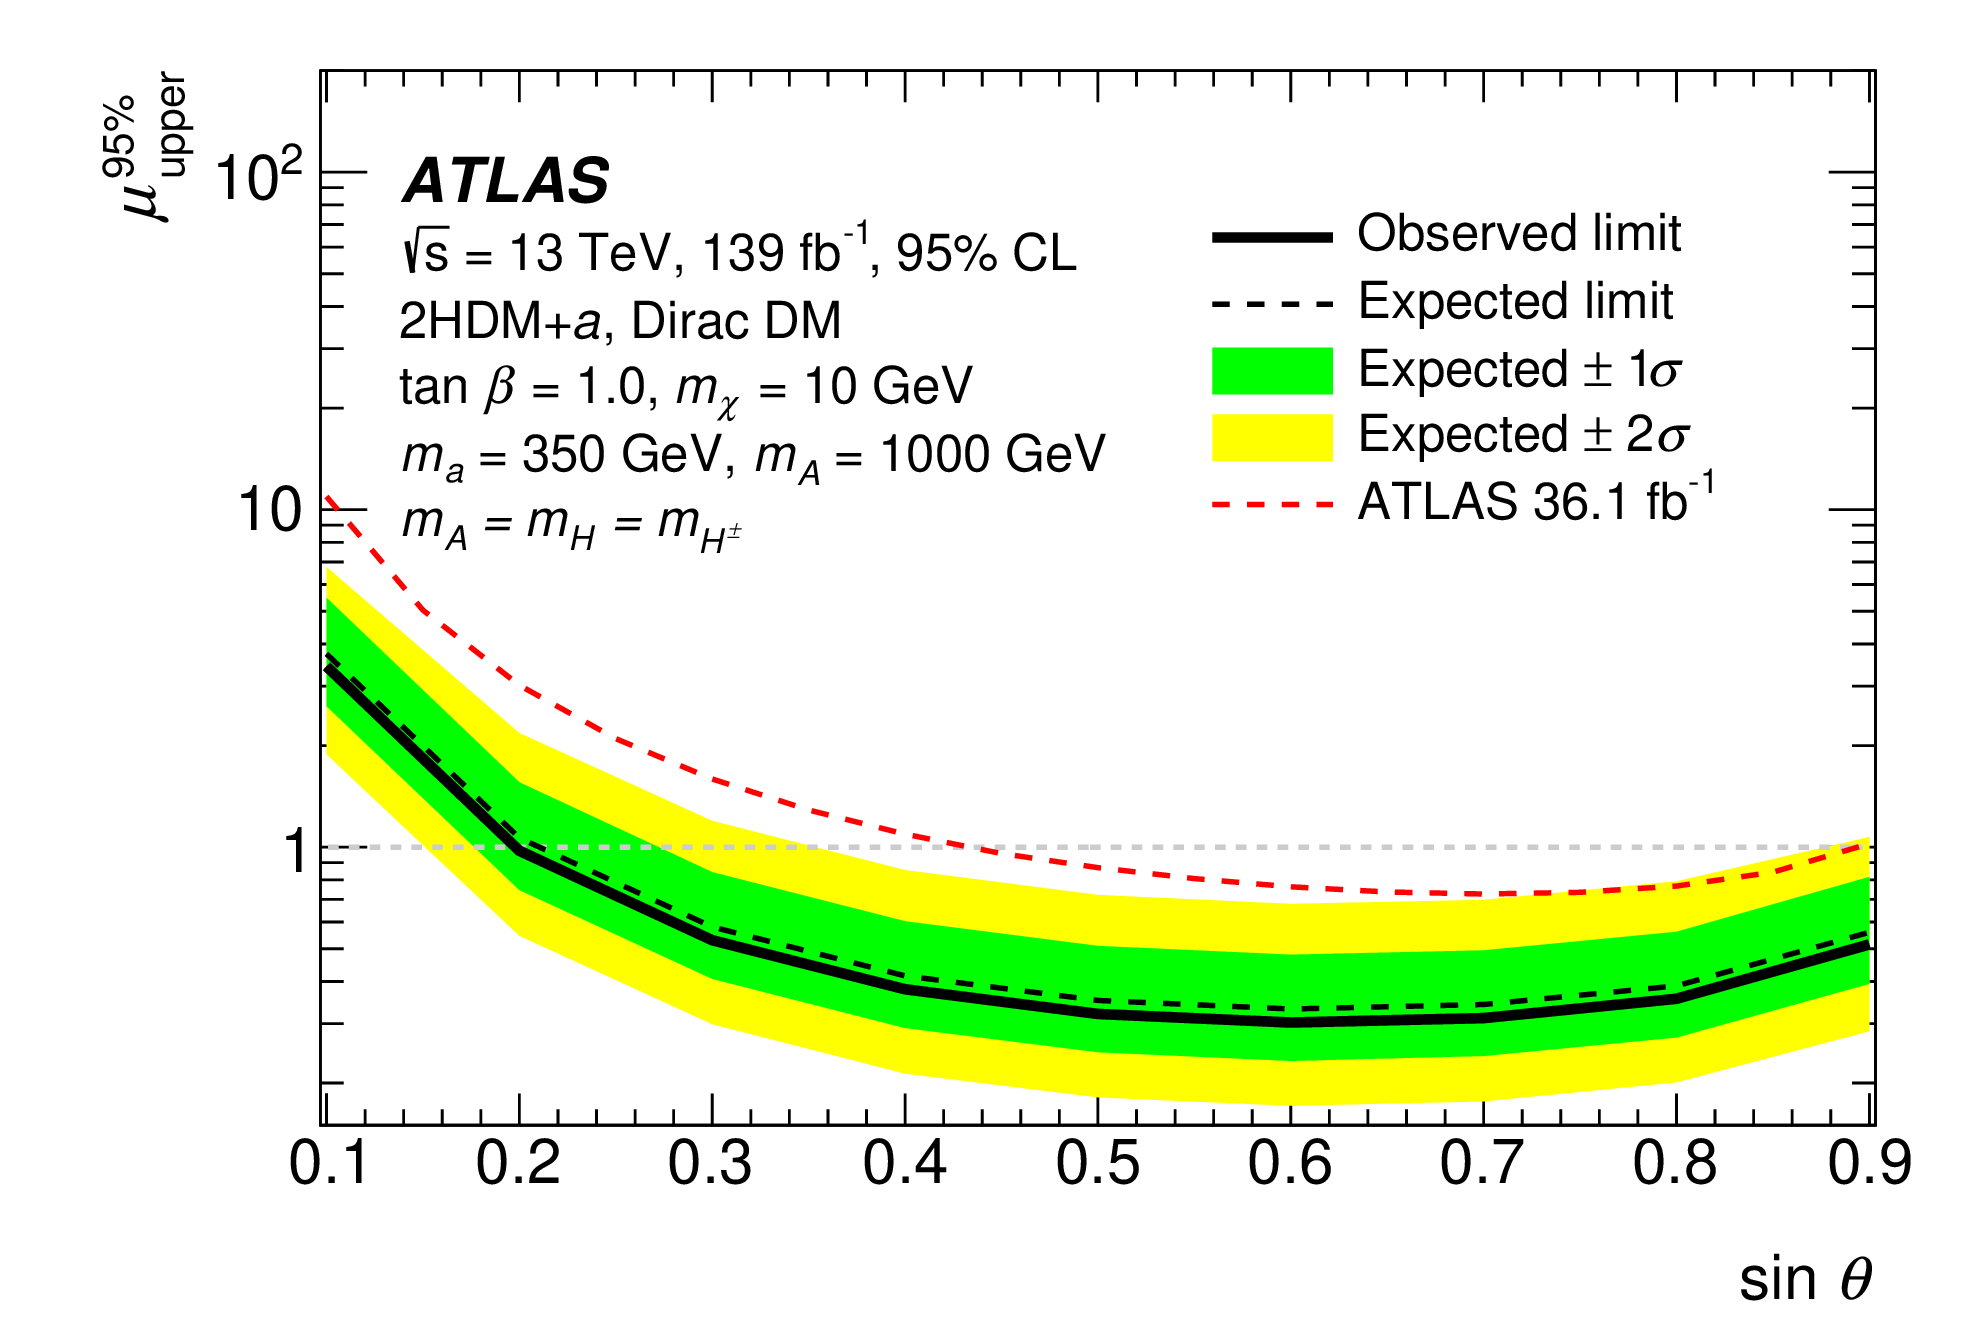
\includegraphics[width=0.49\linewidth]{figures/ch6-DM/fig_06b.png}}  \\    
      
    \caption{$\sin\theta$ exclusion limits for 2HDM+$a$ signals with $\tan\beta = 1.0$ and $m_\chi = 10~\text{GeV}$. The solid black line shows the observed limit, while the dashed black line indicates the expected limit in the absence of signal, with
the corresponding $1\sigma$ and $2\sigma$ uncertainty bands in green and yellow. The dashed red line shows the result from
the $36~\text{fb}^{-1}$ analysis. The region below $\mu_{\text{upper}}^{95\%} = 1$ is excluded at the 95\% CL. In (a), $m_A = 600~\text{GeV}$ and $m_a = 200~\text{GeV}$, while in (b) $m_A = 1000~\text{GeV}$ and $m_a = 350~\text{GeV}$.
    }
    \label{fig:2HDMa-sintheta-limit}
\end{figure}

\subsection{Comparison with Direct Detection Underground Experiments}

In addition to DM searches at collider experiments, extensive DM search programs are also conducted by underground experiments. 
These experiments are designed to detect elastic or inelastic scattering of DM particle candidates, such as weakly interacting massive particles (WIMPs), with atomic nuclei or with electrons in atomic shells of various target materials used in the experiments. 
Such interactions are generally classified as nuclear recoils (NRs) for nucleus scattering and electronic recoils (ERs) for electron scattering. 
A comprehensive review of these experimental techniques can be found in Ref.~\cite{arXiv:2512.23039}.

Figure~\ref{fig:astro-DM} summarizes the upper limits set by the underground experiments on the spin-independent (SI) WIMP--nucleon scattering cross-section as a function of the DM mass. 
The limits obtained from the ATLAS DM search program are translated into constraints on the WIMP--nucleon interaction cross-section to enable direct comparison with results from underground experiments.

\begin{figure}[!htbp]
    \centering
    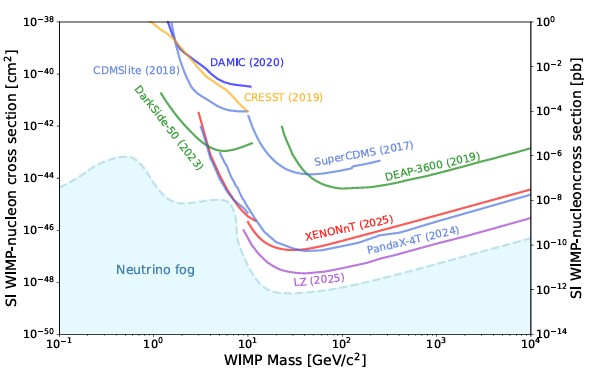
\includegraphics[width=0.9\linewidth]{figures/ch6-DM/astro-xs-DM-mass.jpg}
    \caption{Upper limits on the spin-independent (SI) WIMP--nucleon cross section as a function of DM mass~\cite{arXiv:2512.23039}.}
    \label{fig:astro-DM}
\end{figure}


Within the context of the relevant theoretical models, both the limits on 
$\mathcal{B}(\text{H} \to \text{inv.})$ and those on simplified dark matter (DM) models 
can be compared with results from direct-detection DM experiments. 
For a consistent comparison, limits are expressed at the 90\% confidence level (CL), corresponding to $\mathcal{B}(\text{H} \to \text{inv.}) = 16\%$.

The interpretation of the $\text{H} \to \text{inv.}$ result in terms of the 
WIMP--nucleon scattering cross-section, $\sigma_{\text{WIMP--N}}$, 
within the Higgs portal framework~\cite{ATLAS:2015txa}, 
relies on an effective field theory approach. 
This interpretation assumes that Higgs boson decays into pairs of DM particles are kinematically allowed and that the DM particle is either a scalar or a Majorana fermion~\cite{Eboli:2000ze, Fox:2011fx, DeSimone:2014pda}. 
In this translation, a nuclear form factor of 
$f_N = 0.308 \pm 0.018$ is used.

In simplified DM models, scenarios with an axial-vector mediator are translated into limits on the spin-dependent WIMP--proton scattering cross-section, while vector mediator scenarios correspond to limits on the spin-independent WIMP--nucleon scattering cross-section~\cite{Abercrombie:2015wmb}.

Figures~\ref{fig:xs-DM-mass} and~\ref{fig:xs-Mono-Z-mass} illustrate the complementarity between the collider ATLAS experiment and direct-detection experiments. 
The limits obtained in this analysis are particularly competitive at low DM masses, where experiments based on nuclear recoil measurements typically have reduced sensitivity.

%Figure~\ref{fig:xs-Mono-Z-mass} shows a comparison of the 90\% confidence level (CL) upper limits from direct-detection experiments~\cite{LUX:2017, PandaX-II:2017, XENON1T:2018, XENON1T:2019SD, DarkSide-50:2018, Albert:2017onk, Amole:2019fdf, Wang:2020cgz} with the exclusions obtained in the simplified dark matter (DM) models. 
%The comparisons are presented in the plane of the dark matter mass versus (a) the spin-dependent WIMP--proton scattering cross-section or (b) the spin-independent WIMP--nucleon scattering cross-section~\cite{Boveia:2016mrp}. This analysis, within the context of the simplified models, excludes the region enclosed by the shaded lines.

\begin{figure}[!htbp]
    \centering
    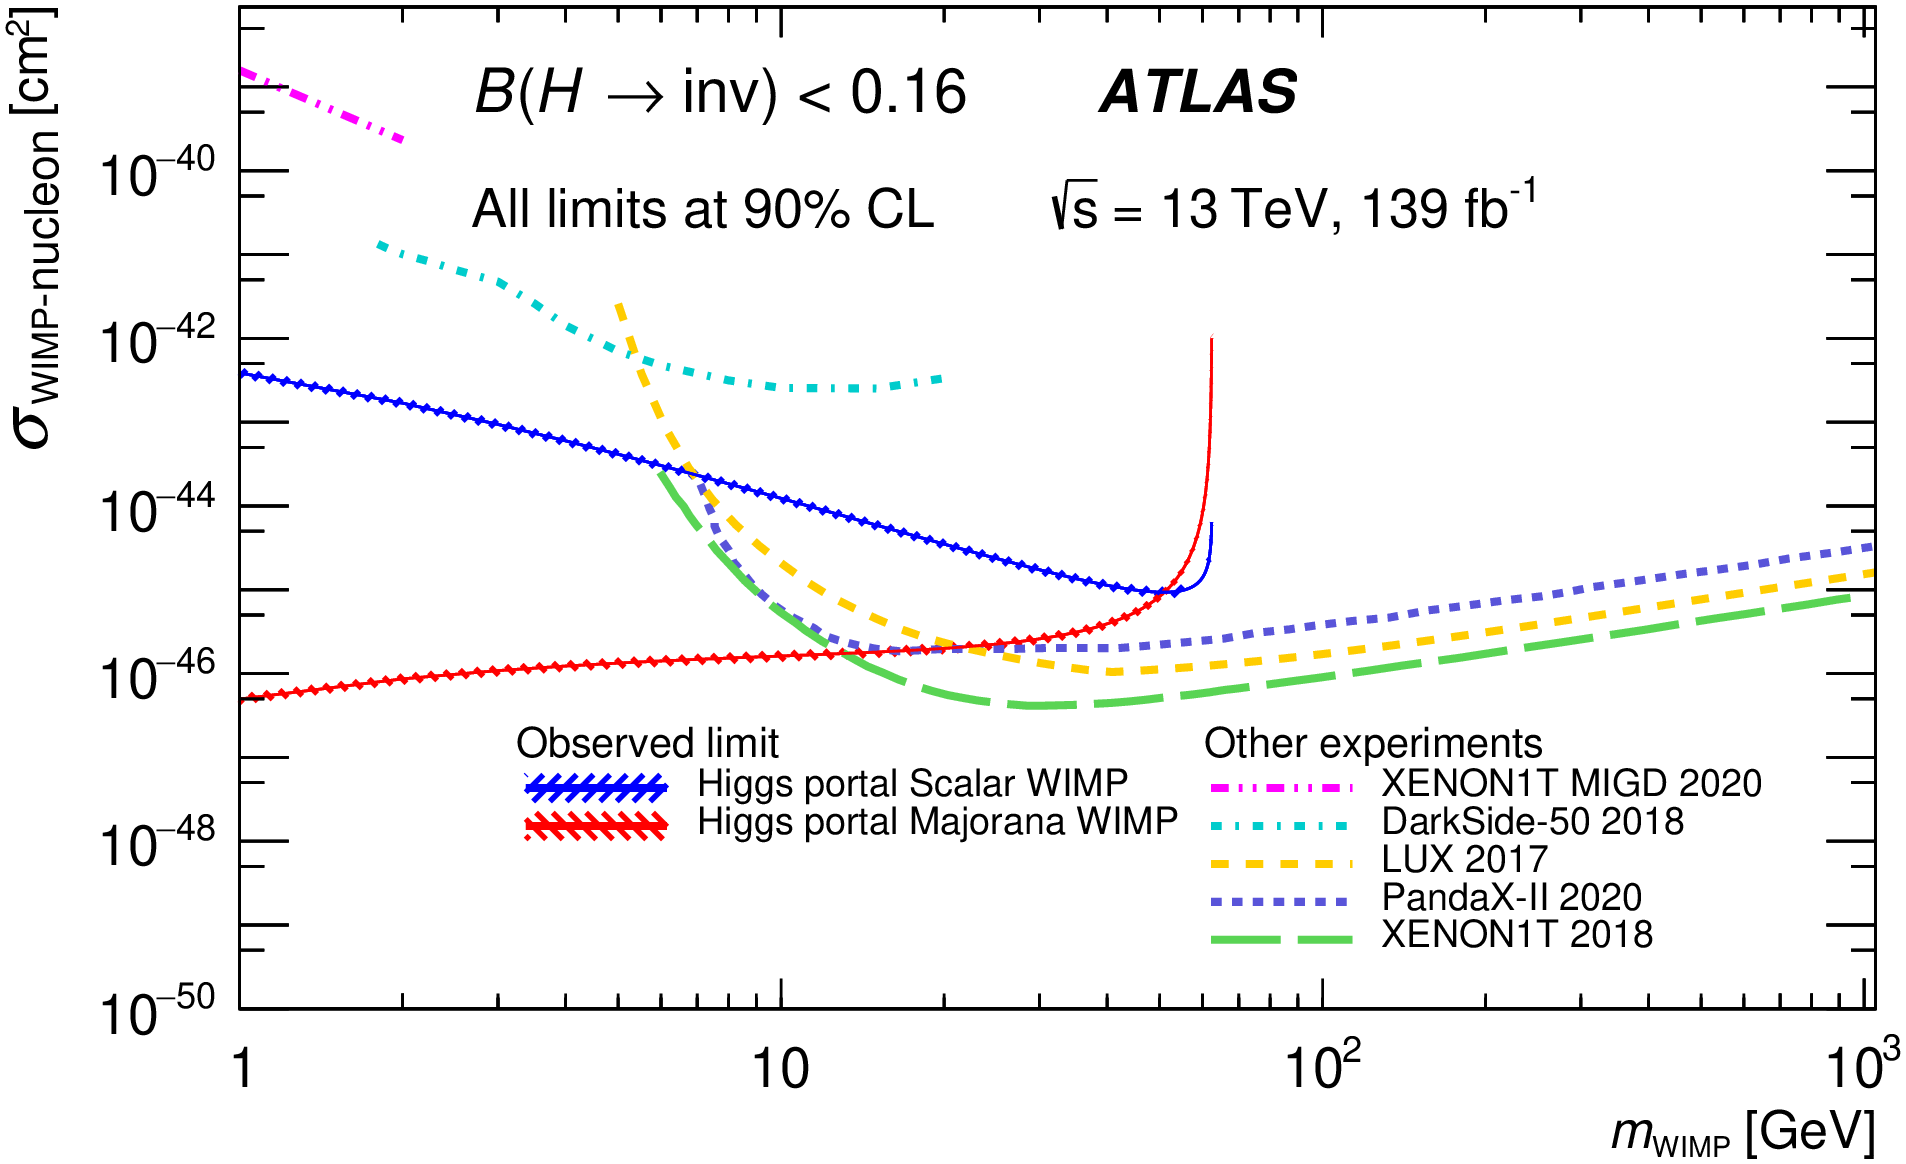
\includegraphics[width=0.9\linewidth]{figures/ch6-DM/fig_07.png}
    \caption{Comparison of the 90\% C.L. upper limits from direct detection experiments~\cite{LUX:2017,PandaX-II:2017,XENON1T:2018,XENON1T:2019SD,DarkSide-50:2018}
    on the spin-independent WIMP--nucleon scattering cross-section with the observed exclusion limits from this analysis as a function of the WIMP mass. The ATLAS interpretation assumes Higgs portal scenarios in which the $125~\text{GeV}$ Higgs boson decays into pairs of dark matter particles~\cite{ATLAS:2016:HinvisibleVBF}, either scalars or Majorana fermions. Uncertainties from the nuclear form factor are shown as a hatched band. Regions above the limit contours are excluded in the $\sigma_{\text{WIMP--N}}$ range shown.}
    \label{fig:xs-DM-mass}
\end{figure}

\begin{figure}[!htbp]
    \centering
    \subfloat[]{
    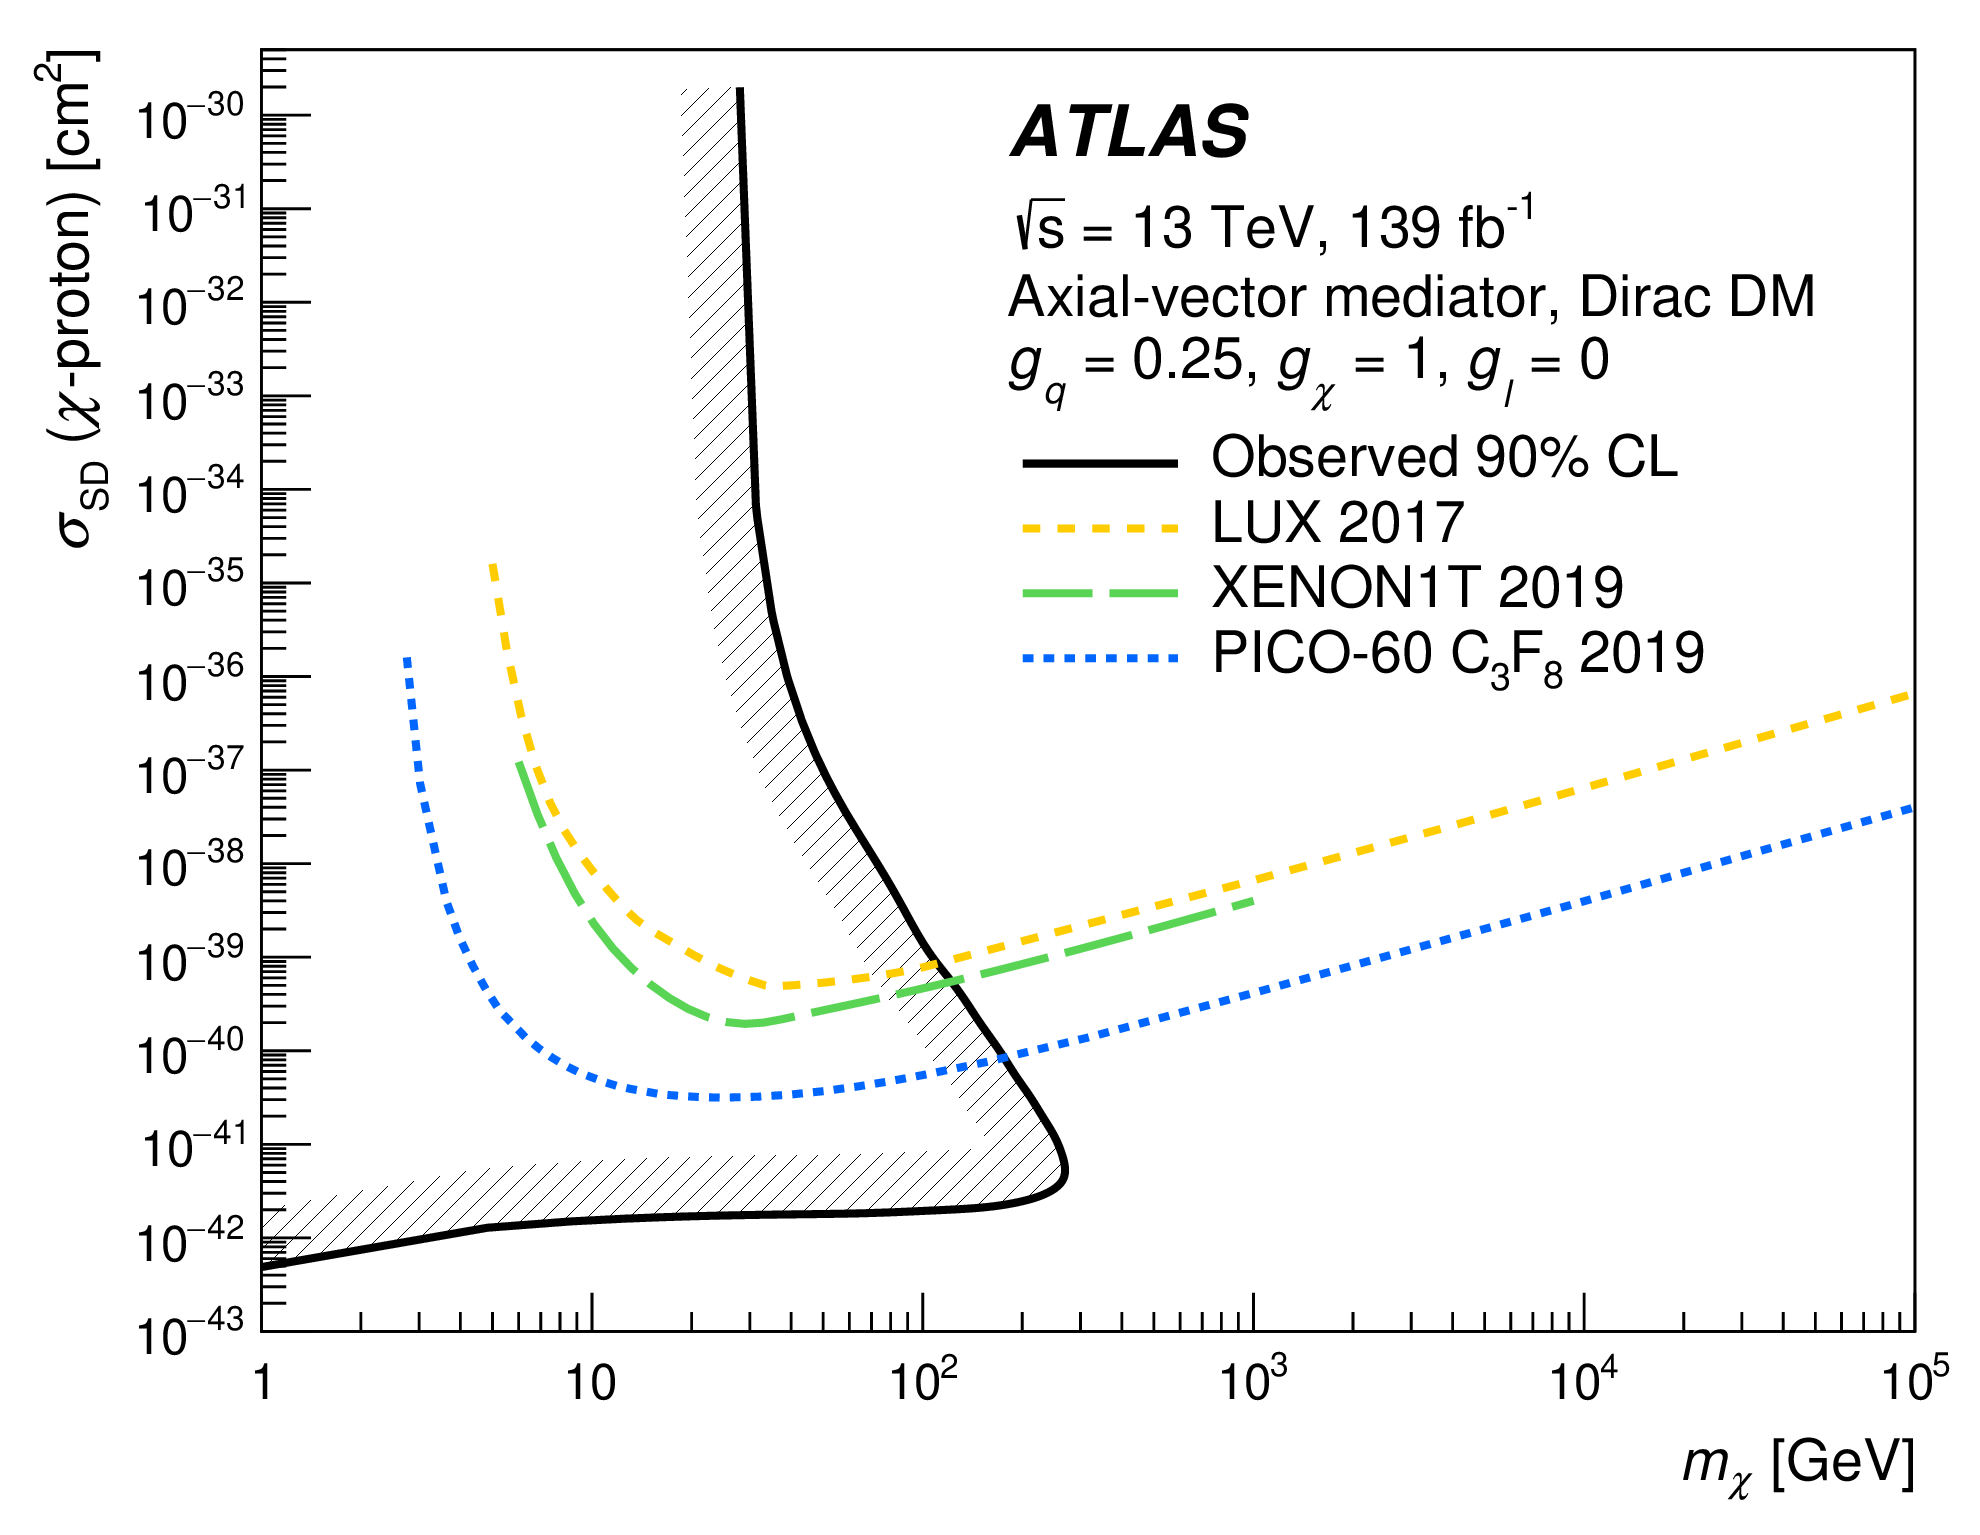
\includegraphics[width=0.49\linewidth]{figures/ch6-DM/fig_08a.png}}
    \subfloat[]{
    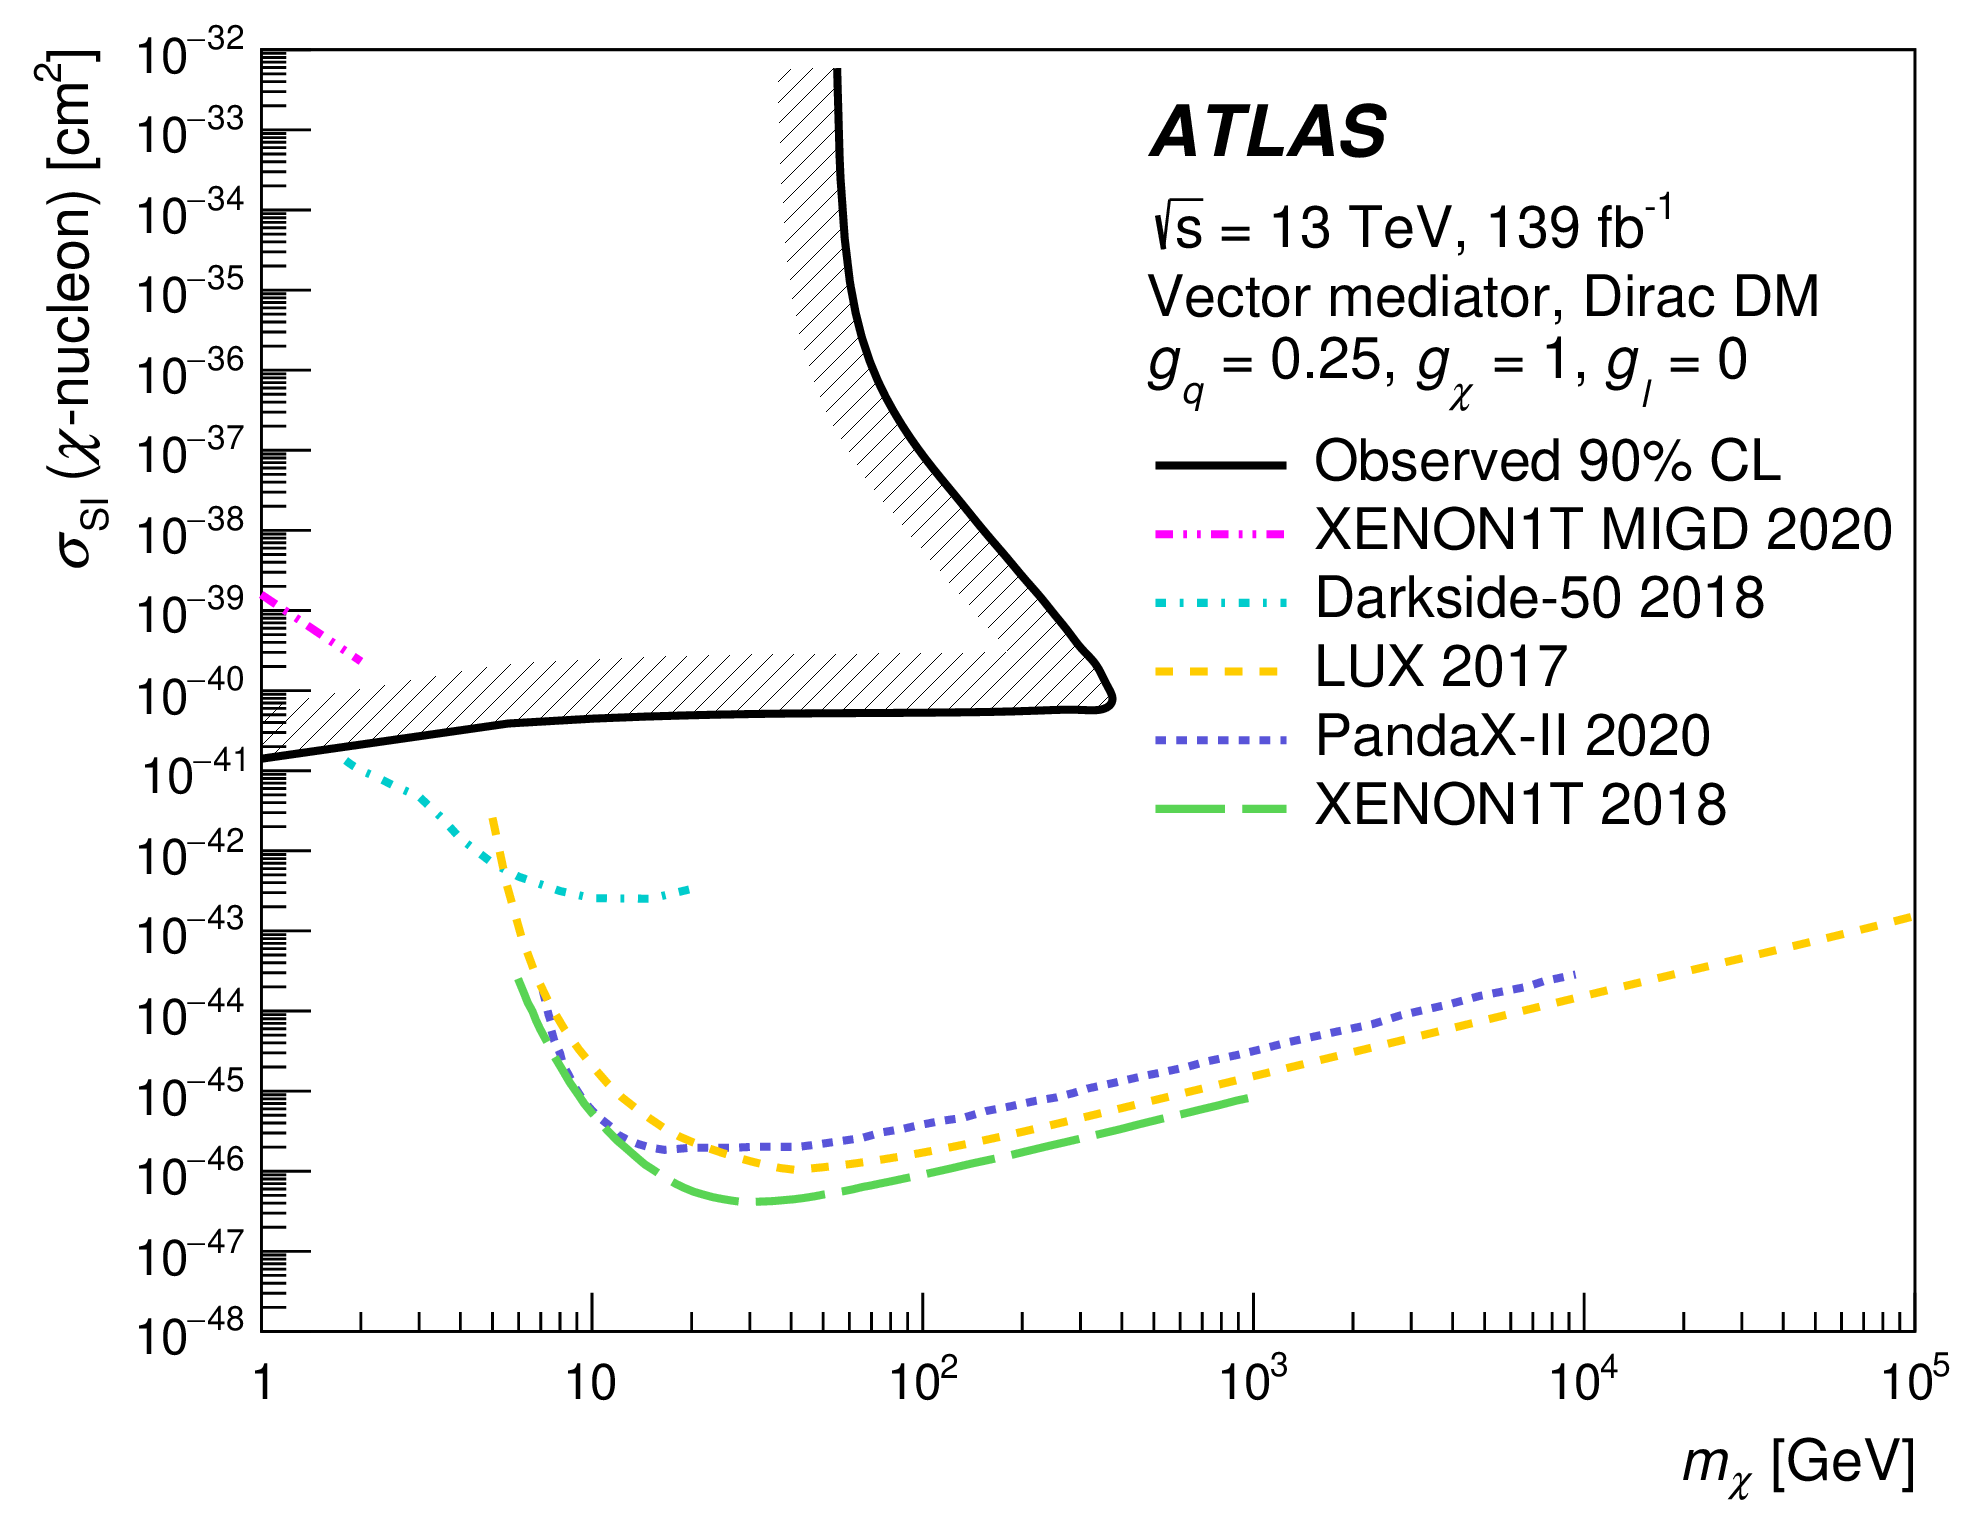
\includegraphics[width=0.49\linewidth]{figures/ch6-DM/fig_08b.png}}  \\    
      
    \caption{Comparison of the upper limits at 90\% CL from direct-detection experiments~\cite{LUX:2017, PandaX-II:2017, XENON1T:2018, XENON1T:2019SD, DarkSide-50:2018, Albert:2017onk, Amole:2019fdf, Wang:2020cgz} with the exclusion obtained in the simplified DM models in the plane of the dark matter mass and (a) the spin-dependent WIMP--proton scattering cross-section or (b) the spin-independent WIMP--nucleon scattering cross-section~\cite{Boveia:2016mrp}. This analysis, in the context of the simplified models, excludes the area within the shaded lines.
    }
    \label{fig:xs-Mono-Z-mass}
\end{figure}

\section{Summary of the DM Search in the $\text{Z} + E_{\text{T}}^{\text{miss}}$ Channel}

Searches for dark matter (DM) using the $\text{Z} + E_{\text{T}}^{\text{miss}}$ final state represent one of the most sensitive channels at the LHC experiments. 
Using the full Run~2 dataset, corresponding to an integrated luminosity of $139~\text{fb}^{-1}$, an upper limit on the branching ratio of the Higgs boson to invisible particles is set to 19\% at the 95\% confidence level (CL). 

Exclusion limits are also derived for simplified dark matter models and 2HDM+$a$ models across several benchmark parameter scenarios. 
The search sensitivity shows a significant improvement compared to previous results obtained using the partial Run~2 dataset corresponding to $36.1~\text{fb}^{-1}$.